%%%%% Definitions of If- toggles
\newif\ifPaperVersion

%\PaperVersiontrue

\newif\ifshowkexamples
\newif\ifshowoldstuff


%%%%% 
%\showkexamplestrue
%\showoldstufftrue

%%%%%
\ifPaperVersion
% Use monochrome?
\documentclass[nolot,nolof,nocover,printed]{fithesis3}
\else
\documentclass[nolot,nolof,cover,digital,color]{fithesis3}
\fi % PaperVersion

\usepackage[T1]{fontenc}
\usepackage[utf8]{inputenc}
\usepackage{cleveref}
\usepackage{hyperref}
%\usepackage{syntax}
\usepackage{amsthm}
\usepackage{mathpartir}
\usepackage{listings}
\usepackage{subcaption}
\usepackage{IEEEtrantools}
\usepackage{xspace} % https://tex.stackexchange.com/a/17873
%\usepackage{todonotes}
%\usepackage{mathtime}

\usepackage[english]{babel}
\usepackage[babel]{csquotes}
\usepackage{float} % floating figures
\usepackage{minted}
\usepackage[toc,page]{appendix}
%\usepackage{amsmath}
%\usepackage{amsfonts}
\usepackage{amssymb} % \rightsquigarrow etc
%\usepackage{makeidx}
%\usepackage{graphicx}

%\usepackage{k}
\usepackage[tight]{k}
%\usepackage{verse}
% For unknown reason, the drawing is too 'white'
%\usepackage[style=math]{k}


\floatstyle{boxed} 
\restylefloat{figure}


%%%%%%%%%%%%%% Thesis metadata %%%%%%%%%%%%%%%
\thesissetup{
title = {An Executable Formal Semantics of C++},
TeXtitle = {An Executable Formal Semantics of C++},
author = {Jan Tušil},
keywords = {C++, semantics, K framework, enumerations, constant expressions, initialization, formal methods},
advisor = {Jan Strejček},
gender = {m},
type = {mgr},
faculty = {fi},
date = {2017/12/12},
assignment = {assignment.pdf, statementOfAnAuthor.pdf},
abstract = {Modern programming languages are expressive, but also complex.
	When a~particular programming language is given a~formal semantics in the framework called \K,
	a~large variety of tools can be derived from it, including an interpreter or a~model checker.
	In this thesis we extend an experimental formal semantics of C++ in \K with a~support for three language features: enumerations, zero-initialization of classes, and compile-time function evaluation. 
	
	The thesis consists of the following parts. First, because \K is not widely known, we provide a~mini-tutorial on how \K can be used to write a~semantics and generate an interpreter of a~simple language. Second, we briefly explain the relevant C++ features from the language point of view. Third, we describe our implementation and its limitations. Fourth, we discuss some defects in major C++ compilers which we found during the implementation effort.
},
thanks = {
 The pages you are looking at would be blank, \\
 were it not for those I now need to thank. \\
 There are too many people under the sun \\
 without whom this work could not be done. \\
 But how to thank them all? I have no clue. \\
 I will try to name here at least a few.\\ % of them
 \\
 First, just under this \^{}\^{}\^{} empty space, \\
 I give my thanks to God, who is full of grace. \\
 And all my family was very supportive; \\
 without them, it would not be so fun to live. \\
 Forgetting about Dwight Guth would be a real shame;\\
 without him, the work would not be the same.\\
 I would also like to thank my advisor, Jan Strejček, \\
 without whom I would not be able to fini\ldots
 }
%bib = {references.bib}
}

% Although there is only one name on the cover...
% Nobody could ever read this text.

% The pages you are looking at would be blank
% if it were not those I need to thank.
% There are just too many people under sun
% without which this work could not be done.

% thank ~ blank
% sun ~ done, one
% those ~ knows
% them ~ poem
% names ~ James, games

%\addbibresource{references.bib}

%% Some math aliases
\newcommand{\var}[1]{\mathit{#1}\xspace}
\newcommand{\kast}{\texttt{kast}\xspace}
\newcommand{\krun}{\texttt{krun}\xspace}
\newcommand{\kompile}{\texttt{kompile}\xspace}
\newcommand{\kdoc}{\texttt{kdoc}\xspace}
\newcommand{\clangKast}{\texttt{clang-kast}\xspace}
\newcommand{\kcc}{\texttt{kcc}\xspace}
\newcommand{\Project}{Project\xspace}
\newcommand{\stdN}[2]{\cite[#2]{#1}\xspace}


% Notes about the 'k' package
% \ka{rule x => y} - inline K in ascii format
% \begin{asciik} rule x => y \end{asciik} - K ascii environment
% Displaying open/closed bubbles
% \kall{1}{2}{3}, \kprefix{1}{2}{3}, \ksuffix{1}{2}{3}, and \kmiddle{1}{2}{3}

\lstset {
	basicstyle=\footnotesize\ttfamily
}

\hyphenation{pa-ra-met-rized}

\begin{document}

\bstctlcite{BSTcontrol}

\chapter{Introduction}

Writing correct software is hard.
%Software verification is hard.
Although formal methods for software verification are being developed, there are only a~few high-quality tools on the market. In order to create a~production-ready tool based on a~particular set of formal methods and targeting a~particular language, it is necessary to understand the formal methods, the precise semantics of the target language, and possibly some other things. Researchers and engineers often work in teams, and various teams often implement different techniques for the same language; because of that, a~platform which would enable component reuse and separation of concerns might significantly improve the productivity of the tool developers.

\K framework is one such platform. It is based on the idea that formal, executable language semantics can be used to derive a~large variety of tools, including interpreters, debuggers, model checkers or deductive program verifiers~\cite{rosu-2017-marktoberdorf} (see Figure~\ref{kidea}). Tool developers skilled in a~particular area of formal methods can work inside their area of expertise and focus on developing language independent tools, while leaving language details to someone else. Thus a~separation of concerns is achieved.

\begin{figure}[ht]
\centering
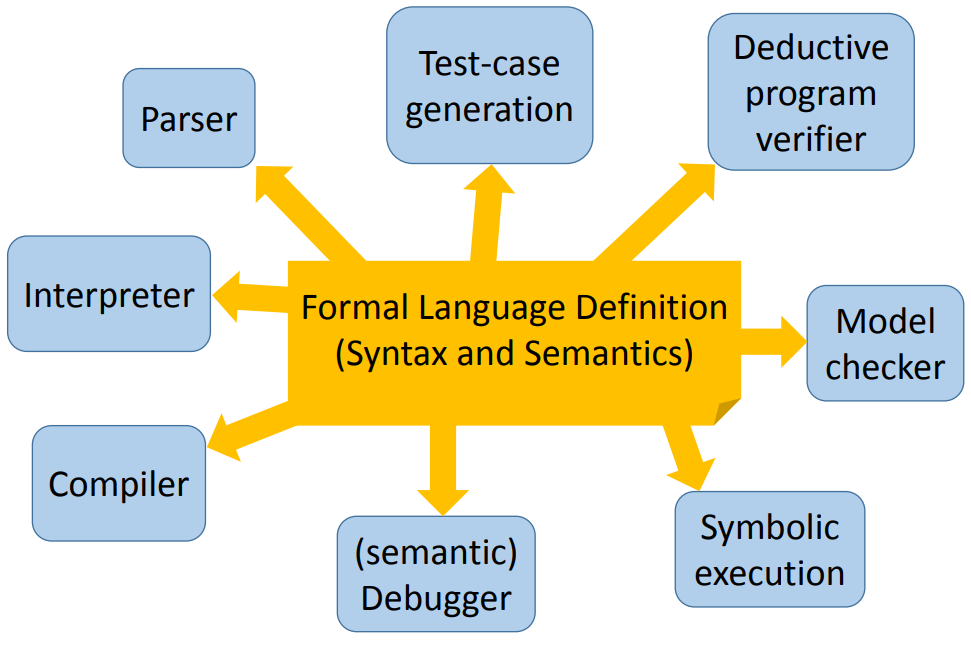
\includegraphics[width=0.7\linewidth]{img/kidea.png}
\caption[The \K idea]{The idea behind \K. Adopted from~\cite{rosu-2015-meseguer}.}
\label{kidea}
% The image is simply print-screen-ed. Je to ok? A muzu rikat, ze jsem ho adoptoval?
\end{figure}

\K framework has been successfully used to give formal semantics to various languages, including Java~\cite{bogdanas-rosu-2015-popl}, Python, Javascript~\cite{park-stefanescu-rosu-2015-pldi}, Agda~\cite{Tokarcik2015}, and C~\cite{ellison-2012-thesis,hathhorn-ellison-rosu-2015-pldi}, all of which is publicly available. The C semantics has been used to create RV-Match, a~\enquote{tool for checking C programs for undefined behavior and other common programmer mistakes}~\cite{guth-hathhorn-saxena-rosu-2016-cav}.  At the time of writing, the C semantics is being extended to support the C++ programming language. The C++ support is also the focus of this thesis. From this point on, when we write \enquote{Project}, we mean this project of defining C/C++ language semantics in \K.

The thesis aimed to implement two language features, \textit{enumerations} and \textit{compile-time evaluation of constexpr functions}, where the latter is an important part of a~language trait called \textit{constant expressions}. When we decided to implement the enumerations, we thought that it is a~relatively simple language feature: they do not have any special runtime behavior, do not interfere much with other language features, and they exist in the language from its beginning. \textit{Scoped enumerations}, introduced in C++11~\cite{ISOcpp11}, are even simpler both from language and user point of view (the legacy C-style enumerations still need to be supported, though). However, a~careful reading of the standard~\cite{n4296} revealed us that the enumerations behave in many ways, some of which we considered to be surprising, as we did not know them from common programming practice.
%TODO tady bych se jeste neodkazova na n4296

\textit{Constant expressions}, on the contrary, had undergone a~deep change in C++11, which allowed a~restricted set of runtime computations to happen in the compilation time; the future revisions released the restrictions to the point that in C++17~\cite{ISOcpp17}, almost arbitrary side-effect free computations can happen in the time of compilation. Because of that, we expected from the beginning that in order to implement the constant expressions (and \textit{compile-time function evaluation} in particular) a~more fundamental change to the semantics would have to be made.

Both features were successfully implemented. The implementation of enumerations is production ready and was largely merged into the upstream; the compile-time function evaluation 
%is not ready for production yet and 
will be probably merged later when the precise semantics of constant expressions is implemented. 
%It went out that the they play together rather nicely: C++ requires enumerators to be initialized with constant expressions; therefore, the implementation of enumerations was used to test the implementation of constant expressions. 
In addition, we fixed several bugs in the Project, including one hard-to-debug nondeterministic behavior, and implemented \textit{zero initialization} for objects of classes types.

%TODO mam v textu rozebrat ten problem zero-inicializace trid?
% (TODO tohle asi prijde dat do vice minuleho casu).
 
%"ukazalo se"
%(TODO zminit, ze za tim je ten 'constexpr' keyword).

The purpose of this text is to describe the implementation of the aforementioned features. It is organized as follows. First, the \K framework is described in such level of detail, which allows a~reader to understand the implementation of the features and which enables her to experiment with simple language definitions. Second, basic concepts of the C++ language are outlined, followed by a~deeper discussion of the selected language features. Third, we explain the general architecture of the \Project. Fourth, the implementation of the language features is described. The final sections of the text contain an evaluation of the implementation, with a~discussion of possible future work.

%TODO Říct, že přehled souvisejících věcí je v tom článku z PLDI'15.
% at first, the project of C/C++ semantics is introduced; then the concepts involved are described in greater depth; then a~general architecture of the project of C/C++ semantics is outlined, followed by a~more detailed description of the parts related to the selected features. A discussion of details of the implementation...

%TODO pouzit figure 2 z PLDI'15, ACM. 2015.


% TODO dat jako prilohu k diplomce virtualku s nainstalovanym prostredim.
% TODO zminit prekazky pri vyvoji: pomala kompilace, nedeterminismus?

\chapter{K framework} \label{chap:k}

This chapter intends to give a~brief overview of the \K framework.
The level of detail here is just necessary to understand the description of implementation in Chapter~\ref{chap:implement}; an inquisitive reader is encouraged to go through the K tutorial\footnote{\url{http://www.kframework.org/index.php/K_Tutorial}}.

%% Taky bych chtel popsat, jake nastroje K framework nabizi, z ceho se sklada apod. Ale ze aktualni prochazi rekonstrukci, takze nektere vlastnosti nefunguji. Pdf dokumentace ze semantiky. Obycejny interpreter, model checker, ...
%


%\paragraph{K And Operational semantics}

%TODO reference some courses and lecture notes for small-step structural operational semantics
%TODO cite the k tutorial.

%TODO rozlisovat mezi 'language definition' - tim budu vzdycky oznacovat konkretni semantiku v K, a~proste semantikou.

In the \K framework, languages are described in a~style commonly known as \textit{operational semantics}. For any language $\var{L}$, when $\var{L}$ is given a~particular definition $\var{D}$ in \K framework, then $\var{D}$ assigns to every program in $\var{L}$ a~transition system $( \var{Cfg}, \rightarrow )$. Here $\var{Cfg}$ denotes a~set of program configurations and $\rightarrow$ is a~binary relation over $\var{Cfg}$; the relation is called a~\enquote{transition relation} and its elements are \enquote{transitions}. %Transitions correspond to computational steps; the existence of a~transition between two given configurations is determined by some kind of deductive system., or by pattern matching rewriting rules to the configurations (in case of \K).

%TODO an image of a~transition system

The configurations are not abstract, but they have an internal structure, which depends on the definition $\var{D}$. For imperative languages, the configurations may consists of a~\enquote{program} part and a~\enquote{data} part.

\section{Terms}

The program part can be represented as a~term. \K allows to define a~multisorted algebraic signature $(S, \Sigma)$, where $S$ is a~set of sorts and $\Sigma$ is an $S^*$-sorted set of symbols; closed terms over this signature form a~(multisorted) term algebra. One may then choose a~particular sort $s \in S$ and declare the set of all programs to be the set of all closed terms of the sort $s$.

\begin{figure}[t]
\begin{lstlisting}
syntax H
syntax H ::= world()
syntax H ::= hello(H,H)
\end{lstlisting}
\caption{Simple syntax definition in \K.}
\label{fig:helloSorts}
\end{figure}

Sorts are defined using \lstinline|syntax| keyword. The definition in Figure~\ref{fig:helloSorts} defines a~sort \lstinline|H| and a~nullary constructor \lstinline|world| and a~binary constructor \lstinline|hello| of that sort. Uknown sorts on the left-hand side of the operator~\lstinline|::=| are automatically defined, and when defining multiple constructors for one sort, the right-hand sides can be chained with the operator~\lstinline{|}{}. The definition above is therefore equivalent to the following definition:
\begin{lstlisting}
syntax H ::= world() | hello(H,H)
\end{lstlisting}
Furthermore, \K allows the sort constructors to be given in an infix syntax and to contain various symbols. Therefore, instead of
\begin{lstlisting}
syntax G ::= unit() | add(G, G) | inv(G)
\end{lstlisting}
it is possible to write
\begin{lstlisting}
syntax G ::= ".G" | G "+" G | "-" G
\end{lstlisting}
to describe the signature of groups. \K also supports subsorting; the following definition makes the sort \lstinline|Int| a~subsort of the sort \lstinline|Real|:
\begin{lstlisting}
syntax Real ::= Int
\end{lstlisting}

\K provides a~set of pre-defined sorts, which include \lstinline|Id| (the sort of C-like identifiers), \lstinline|Int|, \lstinline|Bool|, \lstinline|List|, and \lstinline|Map|. Using these sorts, an algebraic signature of an imperative language can be defined as in Figure~\ref{impSyntax}. From the definition, \textit{arithmetic expressions} (represented by the sort \lstinline|AExp|) are integers, identifiers, and sums of other arithmetic expressions; boolean expressions are boolean constant, comparisons of arithmetic expressions etc.

\begin{figure}[ht]
\begin{lstlisting}
syntax AExp  ::= Int | Id
               | AExp "+" AExp
syntax BExp  ::= Bool
               | AExp "<=" AExp
               | "!" BExp
               | BExp "&&" BExp
               | "(" BExp ")"
syntax Block ::= "{" "}"
               | "{" Stmt "}"
syntax Stmt  ::= Block
               | Id "=" AExp ";"
               | "while" "(" BExp ")" Block
               | Stmt Stmt
syntax Pgm   ::= Stmt
\end{lstlisting}
\caption{A definition of syntax of a~simple imperative language.}
\label{impSyntax}
\end{figure}


\section{Configurations}

A program configuration is a~cell, which can contain nested cell; a~cell 
%A part of a~program configuration can be stored in a~\textit{cell}, which
can be thought of as a~labeled multiset~\cite{hathhorn-ellison-rosu-2015-pldi}. Cells may contain terms of a~given sort or other cells. In a~source code of a~language definition in \K, cells are written in an XML-style notation.

Figure~\ref{impConfiguration} contains a~snippet of such source code. The keyword \lstinline|configuration| here defines three cells (\lstinline|T|, \lstinline|k|, and \lstinline|state|), and an initial configuration of the language. This initial configuration also determines the structure or \textit{shape} of all configurations of the language. Every cell in the definition has some content: the \lstinline|state| cell contains \lstinline|.Map|, which is a~nullary constructor of sort \lstinline|Map|, representing an empty map; the \lstinline|k| cell contains a~term of sort \lstinline|Pgm| consisting of a~variable with name \lstinline|$PGM|, and the \lstinline|T| cell contains the other two cells. The initial configuration for program \lstinline|P| is just like that, except that the variable \lstinline|$PGM| is replaced by a~term representing the program \lstinline|P|.

\begin{figure}
\begin{lstlisting}
configuration <T>
                <k> $PGM:Pgm </k>
                <state> .Map </state>
              </T>
\end{lstlisting}
\caption{A definition of an initial configuration of a~simple imperative language.}
\label{impConfiguration}
\end{figure}

We have said earlier that the programmer may choose a~sort, whose terms will represent the \enquote{program} part of the configuration; that happens in the configuration definition. In this particular language definition, the \enquote{data} part of the configuration is represented by a~term of sort \lstinline|Map|. %Of course, the programmer may choose to use a~configuration with only one cell to represent both


%TODO a~co je toplevel konfigurace?

\section{Implementations of \K}

Before going further, let us note that in the time of writing there exist two implementations of \K: UIUC-\K\footnote{\url{https://github.com/kframework/k}}, developed by University of Illinois in Urbana-Campaign, and RV-\K\footnote{\url{https://github.com/runtimeverification/k}}, developed by RuntimeVerification, Inc. The former is intended to be the reference implementation, the latter is optimized for RV's tools based on the Project. Both implementations provide the same set of command (e.g. \kompile, \krun); however, RV-\K differs from UIUC-\K in several aspects. One of the differences is that the RV-\K requires the configuration to contain a~cell with an \lstinline|exit| attribute: the cell contains the value returned by \krun. Because of that, it does not supports the examples included in the official \K tutorial. However, all examples in this chapter from this point further work with both implementations.

\section{Parsing}
It can be seen from Figure~\ref{impSyntax} that definitions of algebraic signatures in \K looks similar to definitions of context-free grammars using a~BNF notation. This is not a~coincidence. In fact, \K allows to specify the \textit{concrete syntax} with use of special \textit{attributes}. This subsection describes some of the parsing facilities provided by \K. The \Project does not use them, but the description enables the reader to easily experiment with the provided examples.

\begin{figure}
\begin{lstlisting}
module ARITH-SYNTAX
  syntax AExp  ::= Int
                 | AExp "/" AExp              [left]
                 > AExp "+" AExp              [left]
                 | "(" AExp ")"               [bracket]
  syntax Pgm ::= AExp
endmodule
module ARITH
  imports ARITH-SYNTAX  
  configuration <T>
                   <k> $PGM:Pgm </k>
                   <ret exit="">0</ret>
                </T>
endmodule
\end{lstlisting}
\caption{File \protect\path{arith.k}. Note the \lstinline|ret| cell with the \lstinline|exit| attribute.}
\label{arithSource}
\end{figure}

Figure~\ref{arithSource} contains a~definition of a~simple language of arithmetic expressions. The definition contains a~few things we have not described yet. First, it is split into two modules. The \lstinline|ARITH-SYNTAX| module contains everything which is needed to generate a~parser, while the \lstinline|ARITH| module contains everything else. Second, one of the sort constructors is separated from the previous one by the~\lstinline|>| sign. This causes the preceding productions in the concrete syntax grammar to have a~higher priority than the following ones and thus to bind tighter. Third, some constructors have \textit{attributes} attached; the attribute \lstinline|left| causes a~binary constructor to be left-associative, and the attribute \lstinline|bracket| means that the corresponding unary constructor should be parsed as a~pair of brackets.
%TODO mozna se to podoba Parsing Expression Grammar

When stored in a~file with name \path{arith.k}, the definition may be compiled using the \kompile command, provided either by UIUC-\K
\begin{lstlisting}
$ kompile arith.k
\end{lstlisting}
or by RV-\K:
\begin{lstlisting}
$ kompile -O2 arith.k
\end{lstlisting}
The \krun command will use the module \lstinline|ARITH-SYNTAX| to generate a~parser and the module \lstinline|ARITH| to generate an interpreter. The names of the modules used to generated the parser and the interpreter are automatically inferred from the filename, but they can also be specified explicitly using command-line arguments. Both parser and interpreter are stored in a~directory \path{arith-kompiled}.

The compiled definition can be used to parse and execute a~program written in the arithmetic language.
\begin{lstlisting}
$ cat addition.arith
1 + 2 + 3
$ krun addition.arith
<T> <k> 1 + 2 + 3 </k> <ret> 0 </ret> </T>
\end{lstlisting}
The command parses the given source file, creates its initial configuration, walks in the generated transition system until it reaches a~terminal configuration, and pretty-prints it. The generated transition system contains only one configuration (the initial one), as the current language definition of Arith does not have any semantic rules.

The pretty-printing implies that the abstract syntax is \textit{unparsed} back to the concrete one. Therefore, from the output above one can not conclude that the file was parsed in the way programmer intended, as changing the left associativity to the right one (by changing \lstinline|left| attributes to \lstinline|right| ones) would not alter the output. However, \krun can be instructed to output a~textual version of its internal representation:
\begin{lstlisting}
$ krun --output addition.kast
`<T>`(`<k>`(`_+__ARITH-SYNTAX`(`_+__ARITH-SYNTAX`(
#token("1","Int"),#token("2","Int")),#token("3","Int"))),
`<ret>`(#token("0","Int")))
\end{lstlisting}
The output is easily readable for a~machine. However, it is less readable for humans. From the output one can get
\begin{lstlisting}
+( +( 1, 2 ), 3 )
\end{lstlisting}
simply be keeping only the content of \lstinline|k| cell, removing superfluous characters and adding spaces. One can see that this expression, when interpreted as in prefix-notation, correspond to the content of \path{addition.c}. From a~different example in Figure~\ref{arithMixed}, one can see that the division has a~priority over addition and the parentheses bind the tightest.


\begin{figure}
\begin{lstlisting}
$ cat simple.arith
5/2 + (1 + 3) / 2
$ krun simple.arith
<T> <k> 5 / 2 + ( 1 + 3 ) / 2 </k> <ret> 0 </ret> </T>
$ krun --output kast simple.arith
<T>`(`<k>`(`_+__ARITH-SYNTAX`(`_/__ARITH-SYNTAX`(
#token("5","Int"),#token("2","Int")),`_/__ARITH-SYNTAX`(`
_+__ARITH-SYNTAX`(#token("1","Int"),#token("3","Int")),
#token("2","Int")))),`<ret>`(#token("0","Int")))
\end{lstlisting}
\caption{Another example of a~program in the language of arithmetic expressions. The last output corresponds to the expression \lstinline|+( /( 5, 2 ), /( +( 1, 3 ), 2 ) )|}
\label{arithMixed}
\end{figure}

\section{Rules}
So far, the definition of language Arith was able to generate only trivial transition systems with one configuration and no transitions. To generate configurations from the initial one, \K provides a~concept of \textit{semantic rules}. In their simplest version, the rules have the form of $\varphi => \psi$, where $\varphi$, $\psi$ are \textit{patterns} - configurations with free variables, where every variable free in $\psi$ have to be free in $\varphi$. We say that a~pattern $\varphi$ \textit{matches} a~concrete configuration $\var{Cfg}$, when $\varphi$ may be turned into $\var{Cfg}$ by substituting free variables of $\varphi$ with concrete terms. In that case we say that the variables \textit{bind} to the corresponding terms. When $\varphi$ matches a~configuration $\var{Cfg}$, a~transition is generated into a~new configuration $\var{Cfg^\prime}$, which is the result of substituting the free variables of $\psi$ with the bound terms.

\subsection{Basic rules}
For example, the module \lstinline|ARITH| of the language Arith may be extended with the following rule:
\begin{lstlisting}
rule <T><k>I1:Int + I2:Int</k><ret>R:Int</ret></T> 
  => <T><k>I1 +Int I2</k><ret>R</ret></T>
\end{lstlisting}
The left-hand side of the rewriting operator (\lstinline|=>|) contains three free variables (\lstinline|I1|, \lstinline|I2|, \lstinline|R|), all of which required to have a~sort \lstinline|Int|. The variables \lstinline|I1|, \lstinline|I2| are used as the two parameters of the constructor~\lstinline|+|, while the variable \lstinline|R| represents the content of the \lstinline|ret| cell. On the right-hand side, \lstinline|I1| and \lstinline|I2| are given as parameters to built-in function~\lstinline|+Int|, which implements the addition of two integers; the variable~\lstinline|R| is used in the same place as on the left side, thus leaving the \lstinline|ret| cell unchanged.

The compiled definition takes two numbers and adds them together:
\begin{lstlisting}
$ kompile arith.k
$ cat simple.arith
1 + 2
$ krun simple.arith
<T> <k> 3 </k> <ret> 0 </ret> </T>
\end{lstlisting}
Here \krun again printed the final configuration. It is possible to print an $i$-th configuration with use of the \lstinline|depth| switch:
\begin{lstlisting}
$ krun --depth 0 simple.arith
<T> <k> 1 + 2 </k> <ret> 0 </ret> </T>
$ krun --depth 1 simple.arith
<T> <k> 3 </k> <ret> 0 </ret> </T>
\end{lstlisting}

\subsection{Local rewriting}
The semantic rule above applies the rewriting operator (\lstinline|=>|) to whole configuration, although it changes only the content of the \lstinline|k| cell. \K implements a~concept called \textit{local rewriting}, which allows language definition developers to use the rewriting operator inside a~cell or inside a~term. With use of local rewriting, the above rule can be written as:
\begin{lstlisting}
rule <T> <k> I1:Int + I2:Int => I1 +Int I2 </k>
         <ret> R:Int </ret> </T>
\end{lstlisting}
The rule can be even more simplified with use of an anonymous free variable, denoted by an underscore (\lstinline|_|):
\begin{lstlisting}
rule <T> <k> I1:Int + I2:Int => I1 +Int I2 </k>
         <ret> _ </ret> </T>
\end{lstlisting}

It is also possible to use the rewriting operator multiple times in one semantic rule (Figure~\ref{fig:twoRewrites}).

\begin{figure}[ht]
\begin{lstlisting}
rule <T> <k> (I1:Int => 0) + (I2:Int => I1 +Int I2) </k>
         <ret> _ </ret> </T> requires I1 =/=Int 0
rule <T> <k> (0 + I:Int) => I </k> <ret> _ </ret> </T>
\end{lstlisting}
\caption{An addition implemented using two rules. The first of the rules contain two occurrences of the rewrite operator.}
\label{fig:twoRewrites}
\end{figure}
A \lstinline|requires| clause specifies a~side condition of the rule; the rule then can apply only if the condition holds. In this particular example, the rule should not apply if the variable \lstinline|I1| is bound to zero. Without the clause, the rule would be able to apply indefinitely.

 
\subsection{Configuration abstraction}

Semantic rules usually need to be aware only of a~few configuration cells. In \K, the semantics rules have to mention only the cells important for the transition. The \K tool then, from the definition of a~configuration, infers the context in which such local rewriting takes place. The rule for addition can be written as in Figure~\ref{ruleAddInKCell}. Such semantics rules are not only shorter and easier to write, but they are also independent on most of the configuration. Hence, when the structure of a~configuration changes, the rules may remain the same. This feature is called \textit{configuration abstraction}.
%TODO ono to funguje i v pripade, ze mame vetsi nasobnost nekterych bunek


\begin{figure}[ht]
\begin{lstlisting}
rule <k> I1:Int + I2:Int => I1 +Int I2 </k>
\end{lstlisting}
\caption{A rule for addition of two integers.}
\label{ruleAddInKCell}
\end{figure}

\section{Computations}
When creating a~language definition, it is often needed to compute something first, and then use the result of the computation to compute something else. For example, when evaluating an \lstinline|if| statement, the condition has to be evaluated first, and only then the statement can be rewritten to its if-block or else-block. In \K, the notion of \textit{first} and \textit{then} is formalized in terms of \textit{computations} and their \textit{chaining}. Computations have the sort \lstinline|K|; all user-defined sorts are automatically subsorted to \lstinline|K|. Computations can be composed using the~\lstinline|~>| constructor, which is associative. The sort \lstinline|K| has a~nullary constructor \lstinline|.K|, which represents an empty computation and acts as a~unit with respect to~\lstinline|~>|. Thus \lstinline|K| with~\lstinline|~>| and \lstinline|.K| form a~monoid.

In practice, the monoidal structure means that any term consisting of computations and the~\lstinline|~>| constructor behave as a~\textit{chain} of computations, with hidden empty computations everywhere inside. One can then insert a~computation \lstinline|c| to any position in the chain simply by rewriting an empty computation on that position to \lstinline|c|. It also allows replacing the rule of Figure~\ref{ruleAddInKCell} with the rule in Figure~\ref{fig:ruleAddInTopOfKCell} without losing any existing behavior. If the old rule matches a~configuration with a~term \lstinline|C| in the \lstinline|k| cell, then the new rule matches the term \lstinline|C ~> .K|, as the anonymous variable binds to the empty computation. But the new rule matches also the term \lstinline|C| because, due the monoidal structure, configurations \lstinline|C| and \lstinline|C ~> .K| are equal.

\begin{figure}[ht]
\begin{lstlisting}
rule (<k> I1:Int + I2:Int => I1 +Int I2) ~> _</k>
\end{lstlisting}
\caption{A rule for addition in the top of the \lstinline|k| cell.}
\label{fig:ruleAddInTopOfKCell}
\end{figure}

On the other hand, the new rule adds some behaviors, because it matches not only when the \lstinline|k| cell contains exactly an addition of two integers, but also when it contains any sequence of computations, where the first computation is an addition of two integers. The first computation in the list is called \textit{the top}.The parentheses in the new rule are needed, as the constructor \lstinline|~>| binds tighter than the operator~\lstinline|=>|.

% Nerozumim presne, jak funguji ty tri tecky

The rules of the form
\begin{lstlisting}
rule <k> SomeRewritingHere ~> _ </k>
\end{lstlisting}
(for example the rule of Figure~\ref{fig:ruleAddInTopOfKCell}) can be also written as
\begin{lstlisting}
rule SomeRewritingHere
\end{lstlisting}
(i.e. as the rule of Figure~\ref{fig:simpleAdd}).

\begin{figure}[ht]
\begin{lstlisting}
rule I1:Int + I2:Int => I1 +Int I2
\end{lstlisting}
\caption{A really simple rule for addition of two integers.}
\label{fig:simpleAdd}
\end{figure}

\section{Strictness and evaluation strategies} \label{sec:k:strictness}

How to compute the sum of three numbers, say $1 + 2 + 3$? In the language Arith, the constructor \lstinline|+| is left-associative, so the natural approach is to compute $1 + 2$ first, which yields a~result $r$, and then to compute $r + 3$. Although it is possible to write such rules manually, \K provides a~number of tools, which enable the programmer to describe such computations on a~higher level of abstraction.

\subsection{Sort predicates}

For every sort \lstinline|Srt|, \K automatically generates a~\textit{sort predicate} \lstinline|isSrt| of sort \lstinline|Bool|. The predicate takes any term and returns \lstinline|true| if the term is of sort \lstinline|Srt|, otherwise returns \lstinline|false|. One may override the default implementation of a~sort predicate by writing a~custom rule.

So far, the definition of Arith language can not evaluate nested expressions, as the built-in function~\lstinline|+Int| can be applied only on terms of sort Int. Moreover, the left side of the rule of Figure~\ref{fig:simpleAdd} requires the involved terms to be of sort \lstinline|Int|. With use of sort predicates, a~rule
\begin{lstlisting}
rule <l> E1:AExp + E2:AExp => -1 </l>
requires notBool isInt(E1) orBool notBool isInt(E2)
\end{lstlisting}
can be added to the language definition; the rule rewrites a~sum of two terms of sort \lstinline|AExp| to \lstinline|-1|, unless both of the terms have the sort \lstinline|Int|. The \lstinline|notBool| and \lstinline|orBool| are built-in functions; \lstinline|isInt| is a~sort predicate for the sort \lstinline|Int|.


\subsection{Heating/cooling}
Using the information above, a~programmer may use the piece of \K code in Figure~\ref{manualHeatCool} to evaluate nested expressions.
\begin{figure}
\begin{lstlisting}
syntax KItem ::= holdAddR(AExp) | holdAddL(Int)
rule E1:AExp + E2:AExp => E1 ~> holdAddR(E2)
     requires notBool isInt(E1)
rule E1:Int + E2:AExp => E2 ~> holdAddL(E1)
     requires notBool isInt(E2)
rule E2:Int ~> holdAddL(E1:Int) => E1 + E2
rule E1:Int ~> holdAddR(E2) => E1 + E2
rule I1:Int + I2:Int => I1 +Int I2
\end{lstlisting}
\caption{Heating and cooling rules, written manually.}
\label{manualHeatCool}
\end{figure}
The idea here is that the left addend is evaluated first, then the right addend is evaluated and finally, the two integers are added using the built-in function \lstinline|+Int|. One way to interpret the rules is that the first two rules extract an unevaluated expression out of the addition, which creates a~hole in the term, the extracted expression is then evaluated, and the third and fourth rule plug the evaluated expression back into the hole. The constructors \lstinline|holdAddR| and \lstinline|holdAddL| are used to represent the original term without the extracted subterm; the sort \lstinline|KItem| is a~bit special, but it is subsorted to the sort \lstinline|k| as any user-defined sort. The process of extracting a~subterm is known as \textit{heating}, while the opposite process is called \textit{cooling}. 

\subsection{Evaluation contexts}
Heating and cooling rules are very common and also tedious to write manually. In \K, the idea of evaluating a~certain subterm first can be expressed in terms of \textit{evaluation contexts}. With use of keywords \lstinline|context| and \lstinline|HOLE|, the \K code
\begin{lstlisting}
syntax KItem ::= holdAddR(AExp)
rule E1:AExp + E2:AExp => E1 ~> holdAddR(E2)
     requires notBool isInt(E1)
rule E2:Int ~> holdAddL(E1:Int) => E1 + E2
\end{lstlisting}
can be equivalently expressed as:
\begin{lstlisting}
context HOLE:AExp + E:AExp [result(Int)]
\end{lstlisting}
The \lstinline|context| declaration means exactly that: whenever the top of a~\lstinline|k| cell contains an addition of two \lstinline|AExp|s and the first one is not of sort \lstinline|Int| (as specified using the \lstinline|result| attribute), extract the first one, push it on the top of the \lstinline|k| cell and replace the addition with some placeholder; when the extracted subterm gets evaluated to \lstinline|Int|, plug it back to the original context.

With use of context, the code on Figure~\ref{manualHeatCool} can be equivalently expressed as
\begin{lstlisting}
context HOLE:AExp + E:AExp [result(Int)]
context I:Int + HOLE:AExp [result(Int)]
rule I1:Int + I2:Int => I1 +Int I2
\end{lstlisting}
which significantly reduces the amount of code. When compiled, the generated interpreter correctly evaluates the expression $3 + 1 + 7$; the evaluation progress is shown in Figure~\ref{contextEvaluation}.

\begin{figure}
\begin{lstlisting}
3 + 1 + 7
( 3 + 1 ) ~> #freezer_+__ARITH-SYNTAX1_ ( 7 )
4 ~> #freezer_+__ARITH-SYNTAX1_ ( 7 )
4 + 7
11
\end{lstlisting}
\caption{The progress of evaluating the expression $3 + 1 + 7$. An $i$th line represents the configuration after $i$ computational steps, starting from zero. For brevity, only the content of the \lstinline|k| cell is shown.}
\label{contextEvaluation}
\end{figure}

\subsection{Strictness attributes}
\K defines a~sort \lstinline|KResult|, which represents results of computations. When no \lstinline|result| attribute is given to a~context declaration, the declaration behaves as with \lstinline|[result(KResult)]|. When writing a~larger language definition, it is convenient to identify the sorts of desired results and subsort them to \lstinline|KResult|.

\begin{figure}
\begin{lstlisting}
module ARITH-SYNTAX
  syntax AExp  ::= Int
                 | AExp "/" AExp [left, strict]
                 > AExp "+" AExp [left, strict]
                 | "(" AExp ")"  [bracket]
  syntax Pgm ::= AExp
endmodule
module ARITH
  imports ARITH-SYNTAX
  configuration <T>
                  <k> $PGM:Pgm </k>
                  <ret exit=""> 0 </ret>
                </T>
  syntax KResult ::= Int
  rule I1:Int + I2:Int => I1 +Int I2
  rule I1:Int / I2:Int => I1 /Int I2 requires I2 =/=Int 0
endmodule
\end{lstlisting}
\caption{A definition of the language Arith.}
\label{arithFinal}
\end{figure}

When defining a~sort constructor, the constructor may be tagged with an attribute \lstinline|strict|. In that case \K generates a~context declaration for every parameter of the constructor. With use of the \lstinline|strict| attribute, a~definition of the language Arith can be given using only a~few lines (Figure~\ref{arithFinal}).


\section{Functions}

\begin{figure}
\begin{lstlisting}
syntax Int ::= eval(AExp) [function]
rule eval(I:Int) => I
rule eval(E1:AExp + E2:AExp) => eval(E1) +Int eval(E2)
rule eval(E1:AExp / E2:AExp) => eval(E1) /Int eval(E2)
\end{lstlisting}
\caption{An \lstinline|eval| function.}
\label{figAnEvalFunction}
\end{figure}

In the preceding text, a~number of built-in functions was used (e.g. \lstinline|andBool|, \lstinline|=/=Int|, and \lstinline|/Int|). Functions can appear in side conditions (the \lstinline|requires| clause) or on right-hand sides of the rewriting operator. Their application does not create any transitions in the transition system and unlike constructors, functions cannot be pattern-matched. Custom functions can be defined with \lstinline|syntax| keyword and the attribute \lstinline|function|; their behavior is defined using the rewriting operator. See Figure~\ref{figAnEvalFunction} for an example. 
%Since both constructors and functions are defined using \lstinline|syntax| keyword, both of them can be referred to as \textit{syntactic constructs}.

%TODO mohu citovat "A Complete Semantics of K", coz je nejaky tech report, ktery se vali v GitHub repozitari nekoho okolo K?

%TODO Note: in RV-K, the computation chaining seems to work only inside the k cell. I do not know why.


\chapter{C++}

C++ is a~\enquote{general-purpose programming language}~\cite{bjarne-cpp} originally created by Bjarne Stroustrup in the years between 1979 and 1983~\cite{bjarne-faq}. After some time, many independent implementations emerged, and in 1998 the language was standardized as ISO/IEC 14882:1998 international standard (\cite{ISOcpp98}). That version is now known as C++98. The language changed a~lot since that time. New compilers emerged (e.g Clang), compiler developers implemented a~lot of experimental features (e.g. Clang's Modules\footnote{\url{https://clang.llvm.org/docs/Modules.html}}), many defects both in core language and standard library were fixed, and the memory model was standardized. The language is gradually evolving and once in a~while, the C++ Standards Committee~\cite{wg21home} emits an ISO standard. In the time of writing, the newest C++ standard is C++17~\cite{ISOcpp17}, which was technically completed in March 2017 and should be officially published in December 2017.

In this chapter, we describe some fundamentals of the C++ language and those parts of the language relevant to our thesis. Note that the chapter is not intended to be an introduction to the C++ for programmers. Instead, everything is described from the language (and/or a~compiler writer) point of view here.

\section{Standard documents}
The most widely known documents created by the committee are the international standards. However, the committee produces a~large number of documents, most of which are publicly available~\cite{wg21papers}. Every document is assigned a~unique identifier, which is then used to reference the document. Among the publicly available documents are also \textit{workings drafts} of the ISO standard. The working draft is hosted on GitHub\footnote{\url{https://github.com/cplusplus/draft/}} and it is possible to build it directly from its \LaTeX{ }source or to download the emitted releases on the Release page.

In this thesis we mostly use the document \texttt{n4296}~\cite{n4296}, which is the first draft released after the C++14 ISO standard (\cite{ISOcpp14}); this document is also referenced in the source codes of the \Project. We will also refer to the post-C++17 draft \texttt{n4700}~\cite{n4296}, because its wording is much cleaner then C++14's.

%TODO citable project with assigned DOI https://guides.github.com/activities/citable-code/

\section{Fundamentals}

%This section describes some of the fundamental concepts of the C++ language.

In C++, the memory consists of one or multiple sequences of contiguous bytes, where every \textit{byte} has a~unique \textit{address}~\stdN{n4700}{\S 4.4/1}. Various constructs of the language can create and destroy \textit{objects} of some \textit{type}. An object occupies a~region of storage, not necessarily contiguous~\stdN{n4700}{\S 4.5/1}. Objects can contain \textit{subobjects}; an object not contained in any other objects is a~\textit{complete object}. Every complete object has to occupy at least one byte of the storage; therefore, we can think of objects as having an \textit{identity} (we can identify them by the first byte of their storage).

Objects are intended to hold \textit{values}. An object of a~type \lstinline|T| can be represented by a~sequence of \lstinline|sizeof(T)| objects of type \lstinline|unsigned char|; a~value can be represented as a~set of bits~\stdN{n4296}{\S 3.9/4}.
%FIXME: this is not true, see \stdN{n4296}{3.9/4}.
%Although the standard often refers to values, it does not specify what a~\textit{value} is (at least until \cite{n4700}).
One can think of a~value as of a~\textit{datum} together with its \textit{interpretation}, where \textit{interpretation of a~datum} is some concrete, real-world entity\footnote{This notion of \textit{concrete entity} is something different than \textit{C++ entity} as defined in the C++ language~\stdN{n4296}{\S 3/3}. }. 
%Types help to interpret values.
More in-depth discussion about entities and their computer representations can be found in the first chapter of~\cite{progelements}.

%n4700 6.9/4 object representation of an object
%Objects and values.
A \textit{variable} can be either an object or a~\textit{reference}~\stdN{n4700}{\S 6/6}. Reference is not an object; unlike objects, references do not need to occupy storage and do not have an identity.
%Declaration...\stdN{n4296}{\S 3.1/1-2}
%Expressions, value categories \stdN{n4296}{\S 3.10}

An \textit{expression} is a~language construct, which can be evaluated to get a~value and to cause a~side-effect. Every expression has an associated \textit{value category}: it can be either a~\textit{glvalue}, which means that an evaluation of the expression determines an identity of an object (or function or bitfield), or a~\textit{prvalue}, which means that the evaluation initializes an object or computes a~value~\stdN{n4700}{6.10/1}. The category of \textit{glvalue}s is further divided into \textit{lvalue}s and \textit{xvalue}s. 

\section{Enumerations}

Many languages implement enumerated types as a~means for programmers to define a~finite set of related values (as in Figure~\ref{fig:daysInWeek}). Enumerations in the C++ language are based on enumerations from the C language. In this section, we give a~brief presentation of the C++ enumerations, as defined in~\cite{n4296}. Note that this text is concerned with what the language allows, rather than what is considered to be a~good practice. For a~discussion about the latter, we point the reader to the relevant section of CppCoreGuidelines\footnote{\url{http://isocpp.github.io/CppCoreGuidelines/CppCoreGuidelines}}. 

\begin{figure}[ht]
\begin{lstlisting}
enum class Weekday { Monday, Tuesday, /*...*/ };
Weekday next(Weekday d) {
    /* ... */
}
\end{lstlisting}
\caption{Days in a~week.}
\label{fig:daysInWeek}
\end{figure}

\subsection{Unscoped enumerations}

\begin{figure}[ht]
\begin{lstlisting}[language=C++]
enum E { A = 5, B = A + 3 };
enum E e = B;
\end{lstlisting}
\caption{A declaration of an \textit{unscoped enumeration} \lstinline|E| with \textit{unscoped enumerators} \lstinline|A| and \lstinline|B|, followed by a~declaration of a~variable \lstinline|e| of type \lstinline|E|, initialized by the enumerator \lstinline|B|. This code is valid in both C++14 and C99.}
\label{CStyleEnumDeclaration}
\end{figure}

Figure~\ref{CStyleEnumDeclaration} shows a~basic C-style declaration of an enumeration \lstinline|E|, with a~subsequent declaration of an object of the enumeration's type. Both declarations are valid in both C and C++. In C++14, the C-style enumerations are called \textit{unscoped enumerations}. An enumeration may contain an unbounded number of named values, called \textit{enumerators}. Here, \lstinline|E| contains two enumerators: \lstinline|A| and \lstinline|B|. In C++14, enumerators of an unscoped enumeration are called \textit{unscoped enumerators} and they are declared in the scope which contains the enumeration declaration (or, in the terms of the standard, the \textit{enum-specifier}~\stdN{n4296}{\S 7.2/11}). Therefore, it is possible to refer to them simply as in this example.

However, due to this behavior, it is not possible to declare two unscoped enumerations with the same enumerator, in the same scope. It is still possible to create the second enumeration in a~different scope, though. The enumeration may even have the same name, as in the Figure~\ref{fig:collidingEnumerators}. If that happens, the old enumerator is \textit{shadowed} with the new one, but it is still possible to access the old one using the scope resolution operator (i.e. \lstinline|::B| in this example).
\begin{figure}
\begin{lstlisting}
enum E{B};
// enum F{B}; // an error
int main() { 
    enum E{B};
    return (int)B;
}  
\end{lstlisting}
\caption{A declaration of an enumeration with the same enumerator as in an already existing enumeration.}
\label{fig:collidingEnumerators}
\end{figure}


When a~name of an enumeration (or a~struct) is used in C, for example in a~declaration of a~variable of that enumeration type, it is necessary to use the \lstinline|enum| keyword (as in Figure~\ref{CStyleEnumDeclaration}). In C++, this is not necessary, as a~name of an enumeration (\textit{enum-name}) denotes a~type (it is a~\textit{type-name}, see~\stdN{n4296}{Annex A.1}). It is still possible to do it in the C way, though. The type names accompanied by the keyword \lstinline|enum| or \lstinline|struct| (or similar) are called \textit{elaborated type specifiers}~\stdN{n4296}{\S 3.4.4}.

\subsection{Scoped enumerations}

The revision C++11 introduced \textit{scoped enumerations}. They are declared using the phrase \lstinline|enum class| or \lstinline|enum struct|, and enumerators of a~scoped enumeration are called \textit{scoped enumerators}. Scoped enumerations differ from the plain enumerations in a~number of aspects; the most significant difference is what they have their name for: scoped enumerators are declared in the scope of their enumeration~\stdN{n4296}{\S 7.2/11}. Because of that, the enumerators have to be referred to using the scope resolution operator (at least outside the enumeration declaration, see Figure~\ref{fig:scopedEnumDecl}). However, unscoped enumerators can be referred to in the same style as well~\stdN{n4296}{\S 5.1.1/11}.

%In C, enumerators have an integral type; in C++14, the

\begin{figure}
\begin{lstlisting}[language=C++]
enum class E { A = 5, B = A + 3 };
E e = E::B;
\end{lstlisting}
\caption{A declaration of a~\textit{scoped enumeration} \lstinline|E| with \textit{scoped enumerators} \lstinline|A| and \lstinline|B|.}
\label{fig:scopedEnumDecl}
\end{figure}

\subsection{Underlying type}

Every enumeration type has associated an \textit{underlying type}. It is an integral type, which can represent all values of the enumeration; it also defines the size of the enumeration\footnote{Technically, it is more complicated: \url{https://stackoverflow.com/q/47444081/6209703}}. The standard library provides the programmer a~way to find out the underlying type of an enumeration (Figure~\ref{fig:stdUnderlyingType}).

\begin{figure}[ht]
\begin{lstlisting}
#include <type_traits>
enum E {A, B, C};
std::underlying_type_t<E> x = 5;
\end{lstlisting}
\caption{The type of the variable \lstinline|x| is the underlying type of \lstinline|E|.}
\label{fig:stdUnderlyingType}
\end{figure}

An enumeration's underlying type can be explicitly specified~\stdN{n4296}{\S 7.2/5}. This is achieved by appending a~colon followed by the name of an integral type right after the \textit{enum-name} in the declaration, as shown in Figure~\ref{fig:explicityleSpecifiedUnderlyingType}. The usual reason why would anyone want to specify an enum's underlying type is to limit the enumeration's size, perhaps because of hardware constraints. Before C++11, this was often achieved through an extension of a~particular compiler. For example, the GNU GCC compiler provides a~special attribute \lstinline|packed|, which causes an enumeration's size to be as small as possible (Figure~\ref{fig:packedEnum}).

\begin{figure}
\begin{lstlisting}[language=C++]
enum E1 : char {A,B};
enum class E2 : short {C,D};
\end{lstlisting}
\caption{Explicitly specified underlying type.}
\label{fig:explicityleSpecifiedUnderlyingType}
\end{figure}

\begin{figure}
\begin{lstlisting}
enum E { A, B } __attribute__((packed));
\end{lstlisting}
\caption{A packed enum.}
\label{fig:packedEnum}
\end{figure}

If the underlying type of a~scoped enumeration is not explicitly specified, it is automatically defined to \lstinline|int|. All scoped enumerations, as well as unscoped enumerations with explicitly specified underlying type, are said to have a~\textit{fixed underlying type}. This stands in contrast to unscoped enumeration without an explicitly specified underlying type. Their underlying type is not fixed, but it is an \textit{implementation-defined} integral type, which can represent all values of the enumeration~\stdN{n4296}{\S 7.2/7}. That also suggests that the underlying type is not known prior the closing brace of the declaration.

The fact that the standard does not specify the exact underlying type for enumerations whose underlying type is not fixed is also the reason why in pre-C++11 (including C11), the enumerations whose size matters to the programmer have to be declared with use of compiler-specific language constructs (as in Figure~\ref{fig:packedEnum}). Without that, the compiler could simply choose the underlying type (and thus the size) of the enumeration (with respect to some standard-given restrictions); in practice, the chosen underlying type is often \lstinline|int|.

\subsection{Values of an enumeration}

The standard also defines the set of values of an enumeration; those are the values, which can be written or read from an object of the enumeration's type. For an enumeration whose underlying type is not fixed, the set of values limits the choice of the underlying type; it is defined such that the values of all its enumerators and all values between the enumerators are values of the enumeration. The definition is rather technical, though; an inquisitive reader shall find it in~\stdN{n4296}{\S 7.2/8}. For an enumeration with a~fixed underlying type, the values of the enumeration are exactly the values of its underlying type. 

\begin{figure}
\begin{lstlisting}
enum class E { A, B };
E giveMeAnEnum();
int foo(E e) {
	E e = giveMeAnEnum();
	switch(e) {
		case E::A: return 3;
		case E::B: return 42;
	}
	/* Unreachable? Well... */
}
\end{lstlisting}
\caption{The reachability of the last line depends on whether \lstinline|E| has a~fixed underlying type or not.}
\label{fig:enumNotReallyUnreachable}
\end{figure}

This behavior may be a~source of confusion for programmers who do not know this; in past, it certainly was for the author of this text. The programmer may write a~code similar to the one of Figure~\ref{fig:enumNotReallyUnreachable}, which assumes that the value of \lstinline|E| has to be either \lstinline|E::A| or \lstinline|E::B|. This assumption may be justified if the programmer knows the set of values which may be returned from the function \lstinline|giveMeAnEnum|. The programmer may try to go one step further and say: \enquote{If the function \lstinline|giveMeAnEnum| tries to return something different than \lstinline|E::A| or \lstinline|E::B|, than the behavior is already undefined in \textit{that} point; therefore, we do not need to handle that situation in \lstinline|foo|.} Such a~reasoning is flawed, because the function \lstinline|giveMeAnEnum| may return e.g.~\lstinline|static_cast<E>(-117)|, which is guaranteed to be well-defined, because \lstinline|-117| is a~valid value of \lstinline|int|, which is the underlying type of \lstinline|E| here. The programmer's reasoning would be valid if the enumeration \lstinline|E| was a~plain unscoped enumeration without an explicitly specified underlying type (i.e.~if we removed the \lstinline|class| keyword). We will not go into detail here, as the reasoning would depend on the technical parts of~\stdN{n4296}{\S 7.2/8}.

\subsection{Enumerators}\label{sec:enumerators}

Declaration of an enumerator may contain an optional \textit{initializer}, which has to be implicitly convertible to an integral type\footnote{It is more complicated, but this is enough here.}. If the initializer is not specified, the value of the enumerator is zero if it is the first enumerator; otherwise, it is the value of the previous enumerator plus one. When an enumeration is fully defined (i.e. \enquote{following the closing brace of an enum-specifier}), the type of each enumerator is the type of the enumeration~\stdN{n4296}{\S 7.2/5}. For example, in the declaration of variable \lstinline|E| in the Figure~\ref{fig:scopedEnumDecl}, the type of the expression \lstinline|E::B| is \lstinline|E|.

\begin{figure}
\begin{lstlisting}
enum E { A };
void foo(int){}
void goo() {
    foo(A);
    foo(E::A);
    foo(E::A+1};
}
\end{lstlisting}
\caption{Unscoped enumerations can be implicitly converted to \lstinline|int|.}
\label{fig:unscopedEnumToInt}
\end{figure}


This is different from C, where enumerators have the type \lstinline|int|. Still, in C++, unscoped enumerations can be implicitly converted to \lstinline|int|~\stdN{n4296}{\S 7.2/10}, so they behave somewhat similarly to C (Figure~\ref{fig:unscopedEnumToInt}). This conversion does not work for scoped enumerations. The other conversion (from integer types to enumerations) is not defined neither for scoped nor unscoped enumerations (Figure~\ref{fig:noConversionFromIntToEnum}).

\begin{figure}
\begin{lstlisting}
enum E { A };
void foo(int x) { E e = x; }
\end{lstlisting}
\caption{This is a~valid C code, but a~C++ compiler would not compile it. The C++ language does not allow an implicit conversion from int to enum. }
\label{fig:noConversionFromIntToEnum}
\end{figure}

An initializer of an enumerator may refer to previously declared enumerators of the same enumeration (see Figure~\ref{fig:scopedEnumDecl}). Inside the enumeration declaration (prior its closing brace), the type of its enumerators is not the type of the enumerator, but always an integral type\footnote{We discuss this in more detail in Chapter~\ref{chap:defects}.}.
%Because of the stronger-than-C type system,
In some cases, it would be even inconvenient if the types of enumerators were types of their enumerations. For example, the declaration in Figure~\ref{fig:scopedEnumDecl} declares an enumerator \lstinline|B| with the initializer \lstinline|A + 3|. If the type of \lstinline|A| in this expression were \lstinline|E|, then the expression would be ill-formed. Scoped enumerations do not convert to \lstinline|int|, therefore the enumerator \lstinline|A| could not be added to an \lstinline|int|.

%
%\begin{figure}
%\begin{lstlisting}[language=C++]
%enum E { A, B = A, C = +A };
%\end{lstlisting}
%\caption{Quiz: what are the types of B and C prior the closing brace?}
%\label{fig:enumeratorTypeQuiz}
%\end{figure}
%

\subsection{Incomplete types}
Some types cannot be used to define objects; those are called \textit{incomplete}~\stdN{n4296}{\S 3.1/5}. A type may be incomplete at one point and complete at another point in a~translation unit. Incomplete types are still useful; they may be used in function declarations to denote its parameters and return values, to define objects of pointer type or references. There are two categories of incomplete types: void types (e.g. \lstinline|volatile void|) and incompletely-defined types. It is not allowed to apply the operator \lstinline|sizeof| to an incomplete type. A programmer may choose to use incompletely-defined types to limit the number of dependencies between header files. An enumeration whose underlying type is not fixed is incomplete until the closing brace of its declaration.

\subsection{Opaque enumerations}

Enumerations with fixed underlying type can be declared \textit{opaque}, that is, without the list of enumerators (see Figure~\ref{fig:opaqueEnumDeclarations}). An enumeration declared using an \textit{opaque-enum-declaration} is a~complete type (it is not an incomplete type); therefore, it can be used almost as a~fully declared enumeration, except that its enumerators are not available. Such an enumeration needs to have a~fixed underlying type (see Figure~\ref{fig:opaqueEnumNotFixedUT}). An opaque enumeration can be fully redeclared later in the program~\stdN{n4296}{\S 7.2/3}.

\begin{figure}
\begin{lstlisting}[language=C++]
enum E1 : char;
enum class E2 : unsigned int;
enum class E3;
\end{lstlisting}
\caption{\textit{Opaque-enum-declaration}s.}
\label{fig:opaqueEnumDeclarations}
\end{figure}

\begin{figure}
\begin{lstlisting}[language=C++]
enum E;
\end{lstlisting}
\caption{Not a~valid declaration, because \enquote{opaque-enum-declaration declaring an unscoped enumeration shall not omit the enum-base}~\stdN{n4296}{\S 7.2/2}}
\label{fig:opaqueEnumNotFixedUT}
\end{figure}

%
%\begin{figure}
%\begin{lstlisting}[language=C++]
%enum class E : short { A, B = A + 2, C };
%\end{lstlisting}
%\caption{Prior the closing brace, the enumerators \lstinline|A|, \lstinline|B| and \lstinline|C| have a~type \lstinline|short|.}
%\end{figure}
%
%\begin{figure}
%\begin{lstlisting}[language=C++]
%enum E { A, B, C = (char)255, D };
%\end{lstlisting}
%\caption{Prior the closing brace, the enumerators \lstinline|A|, \lstinline|B| and \lstinline|D| have an unspecified type, the enumerator \lstinline|C| has type \lstinline|char|.}
%\end{figure}
%
%\begin{figure}
%\begin{lstlisting}[language=C++]
%enum { A };
%enum : char { B, C };
%\end{lstlisting}
%\caption{\enquote{The optional identifier shall not be omitted in the declaration of a~scoped enumeration}(7.2/2), however, it may be omitted in the declaration of an unscoped enumeration.}
%\end{figure}
%

%TODO spoustu veci neprojde uz pres clang-kast
%TODO where is the exact point of declaration?
%TODO inicializer je jednou 'integral constant expression' a~podruhe 'converted constant expression'.

\section{Initialization} \label{chap:lang:init}
As a~part of this thesis, we also implemented a~language feature called \textit{zero initialization} on class types. In this section, we describe how variables are initialized in general, and how \textit{zero initialization} fits into the overall scheme. The details of how we implemented \textit{zero initialization} are present in Section~\ref{chp:implZeroInit}.

\subsection{Initialization forms}
When an identifier is being declared, an \textit{initializer} can be used to specify an initial value of the identifier~\stdN{n4296}{\S 8.5/1},~\stdN{n4700}{\S 11.6/1}. Initializers have many syntactical forms, all of which are shown in Figure~\ref{fig:initializers}. The form of initialization \lstinline|T x(a);| or \lstinline|T x{a};| is known as \textit{direct initialization}~\stdN{n4296}{\S 8.5/16}; this form is used in the declarations of variables \lstinline|a| and \lstinline|b| in the Figure~\ref{fig:initializers}.

An initialization of the form \lstinline|T x{...};| or \lstinline|T x = {...}| (where the ellipsis is a~meta-character indicating a~comma-separated list) is known as \textit{list-initialization}, where the former is \textit{direct-list-initialization} and the latter \textit{copy-list-initialization}. In the Figure~\ref{fig:initializers}, the variables \lstinline|b| and \lstinline|g| are \textit{direct-list-initialized} and the variables \lstinline|d|, \lstinline|h| \textit{copy-list-initialized}. The brace-enclosed comma-separated list is called \textit{braced-init-list}; the initialization in declarations of the form \lstinline|T a = E;| is known as \textit{copy-initialization}.

\begin{figure}[ht]
\begin{lstlisting}
int a(1);
int b{2};
int c = 3;
int d = {4};
int e{};
int f();
char g[]{'a', 'b'};
int h[3] = {1,2,3};
\end{lstlisting}
\caption[Declarations and initializers]{Declaration of variables \lstinline|a|,\lstinline|b|,\lstinline|c|,\lstinline|d|,\lstinline|e|,\lstinline|g|,\lstinline|h|. The identifier \lstinline|f| is not declared as a~variable of type \lstinline|int|, but as a~function taking no parameters and returning an \lstinline|int|.}
\label{fig:initializers}
\end{figure}

It is important to note that all the previous categories consider only the form of the declaration; the semantics of such declarations heavily depends on the types involved. For example, the \textit{copy-initialization} form is often used in a~declaration of a~reference, and when it is used in a~declaration of an object of a~class type, it may invoke \textit{move constructor} as well as a~\textit{copy constructor}.

%TODO inicializace muze probihat i jindy


\subsection{Aggregates}

The C++ language enables programmers to declare \textit{classes}. From the programming methodology standpoint, not all classes are the same kind: for example, some classes are designed to hold values (e.g. \lstinline|std::complex|); other ones encapsulate behavior and while the identities of their instances are really important to programmers, their values are not. Classes can also be categorized from another perspective: some of them maintain a~non-trivial \textit{invariant}, thus restricting the set of possible values their member variables may hold (e.g. \lstinline|std::vector|); other classes consider their members to be independent of each other (e.g. \lstinline|std::pair|), and the set of possible values of such class is then equal to the Cartesian product of the possible values of its members. Such types are commonly known as \textit{product types}\footnote{More formal treatment of product types can be found in~\cite[Chapter~1.5]{hottbook}.}. In C++, the notion of types composed freely from other types is present in the form of \textit{aggregates}:
\begin{displayquote}[\stdN{n4296}{\S 8.5.1/1}]
An aggregate is an array or a~class (Clause 9) with no user-provided constructors (12.1), no private or
protected non-static data members (Clause 11), no base classes (Clause 10), and no virtual functions (10.3).
\end{displayquote}

\subsection{Aggregate initialization}
In newer versions of the language, the restrictions on aggregate classes are more relaxed. For example, an aggregate class may have a~base class, but only under the condition that the base class is non-virtual and public~\stdN{n4700}{\S 11.6.1/1}. Nevertheless, the idea is still the same: an \textit{aggregate} is just something created by a~natural composition of other things. Because of that, the language provides a~special way to initialize an object of an aggregate type - an \textit{aggregate initialization}.

\begin{figure}[ht]
\begin{lstlisting}
struct S {
  char a;
  int b[2];
  double c;
};
S s = {'a', {2, 3}};
\end{lstlisting}
\caption[Aggregate initialization.]{An exaple of an aggregate initialization. The member \lstinline|c| is initialized with the value of the expression \lstinline|double\{\}| , which is a~floating-point zero.}
\label{fig:aggrInit}
\end{figure}
%TODO short captions for the 'List of Figures'


The \textit{aggregate initialization} happens when an aggregate is initialized using \textit{list-initialization}. If it happens, the \textit{elements} of the aggregate, that is, the array elements or the non-static member variables, are initialized with the respective \textit{initializer clauses} in the order of increasing indices, or in the order of declarations, respectively~\stdN{n4296}{\S 8.5.1/2}. If there are not enough initializer clauses in the initializer list, the remaining aggregate elements are initialized from an empty initializer list (see Figure~\ref{fig:aggrInit}).

\subsection{Value initialization}

When an object is created with no initializer, it is \textit{default-initialized}, which in many situations means that no initialization is performed and the object has an indeterminate value. The language also defines a~\textit{value initialization}, whose purpose is to somehow complement the notion of default-initialization:
\begin{displayquote}[\stdN{n4296}{\S 8.5/8}]
\textelp{} An object that is value-initialized is deemed to be constructed and thus subject to provisions of this International Standard applying to \enquote{constructed} objects, objects \enquote{for which the constructor has completed,} etc., even if no constructor is invoked for the object’s initialization.
\end{displayquote}

A value-initialization is performed in various different cases. For example, the standard says
\begin{displayquote}[\stdN{n4296}{\S 8.5/11}]
An object whose initializer is an empty set of parentheses, i.e., (), shall be value-initialized.\textelp{}
\end{displayquote}
which is demonstrated in Figure~\ref{fig:valueInitMember}. (However, the declaration of \lstinline|f| in Figure~\ref{fig:initializers} does not declare an object, but a~function; in that case, no value initialization is performed.) Value initialization is also performed for list-initialized objects of a~class type with a~default constructor~\stdN{n4296}{\S 8.5.4/5.4}. Such class types are not aggregates, so no aggregate initialization can happen for them.

\begin{figure}[ht]
\begin{lstlisting}
struct A {
  T m;
  A():m() {}
};
\end{lstlisting}
\caption{A \textit{value-initialization} of a~member variable in a~constructor.}
\label{fig:valueInitMember}
\end{figure}

To value-initialize an array means to value-initialize all its elements, and to value-initialize an object of a~non-class non-array type means to zero-initialize it. Value initialization of an object of a~class type performs default-initialization; the default-initialization is preceded by zero initialization if the class does not have a~user-defined or deleted default constructor.

\begin{figure}
\begin{lstlisting}
struct A {
  int m;
};
struct B {
  virtual ~B(){}
  int m = 1;
  int n;
};
int bar() {
  A a{};
  B b1{};
  B b2;
  int c{};
}
\end{lstlisting}
\caption{Initialization from an empty initializer list.}
\label{fig:valueInit}
\end{figure}

The source code in Figure~\ref{fig:valueInit} can serve as an example. The variables \lstinline|A|, \lstinline|b1| and \lstinline|c| are list-initialized, while the variable \lstinline|b2| is default-initialized; however, the meaning of the list-initialization among the variables differs. The variable \lstinline|c| is value-initialized, and since it has a~non-class non-array type, it is zero-initialed; after the initialization, the value of \lstinline|x| is zero. The variable \lstinline|A| is aggregate-initialized because class \lstinline|A| is an aggregate; since the initializer-list is empty, its member variable \lstinline|m| is initialized with the initializer \lstinline|{}|, which performs zero-initialization as in the previous case. At the end, the integer \lstinline|a.m| has the value of zero.

The variable \lstinline|b1| is not aggregate-initialized, as the class \lstinline|B| is not an aggregate because it has a~virtual member function (the destructor); the variable \lstinline|n2| is value-initialized instead. The value-initialization performs a~zero-initialization because class \lstinline|A| has neither user-provided nor deleted default constructor, but the default constructor is implicitly-generated. After the zero initialization, a~default-initialization happens, which runs the implicitly-generated default constructor. At the end, the value of \lstinline|b1.m| is one and the value of \lstinline|b1.n| is zero.
In contrast, the variable \lstinline|b2| is only default-initialized; the value of \lstinline|b2.m| is one as in the previous case, but the value of \lstinline|b1.n| indeterminate.

\subsection{Zero initialization}
The exact meaning of \textit{zero-initialization} is described in~\stdN{n4296}{\S 8.5/6}. References are not initialized at all, scalars are initialized to the value of zero converted to the particular scalar type, arrays are zero-initialized element-wise and objects of non-union class types are zero-initialized by zero-initializing all non-static data its members, base class subobjects and padding. We do not deal with union classes in this thesis.

In addition to the cases described in the previous paragraphs, zero initialization also happens in two another situations.
\begin{itemize}
\item When initializing a~character array with a~string literal that is not long enough, the rest of the array is zero-initialized.
\item Before other initializations of variables with non-static storage duration. Programmers may know this in a~simplified form as a~rule \enquote{in C/C++, global variables are initialized to zero}.
\end{itemize}
This thesis is not concerned with these two situations.

\section{Generalized constant expressions}
%This sections describes 

In C++, expressions are used almost everywhere. However, not every kind of expression can be used everywhere: one can hardly imagine the code in Figure~\ref{fig:getcharInEnum} to be valid. The expressions used in an enum declaration or as a~\textit{case} label of a~\lstinline|switch| statement have to be computable in the compilation time. Expressions of that kind are generally known as \textit{constant expressions}; they are defined in~\stdN{n4296}{\S 5.20}.

\begin{figure}
\begin{lstlisting}
enum class E { A = getchar() };
\end{lstlisting}
\caption{A \enquote{wild} expression in a~context that requires a~constant expression. This is not a~valid C++ code.}
\label{fig:getcharInEnum}
\end{figure}

\subsection{Constexpr}

The language contains a~specifier \lstinline|constexpr|, which can be used in some declarations of functions and variables~\stdN{n4296}{\S 7.1.5}. The use of this specifier in a~declaration means that the value of the declared entity can be used in a~constant expression. Of course, the language imposes some restrictions on such entities. When a~variables is declared as \lstinline|constexpr|, its initializer has to be a~constant expression, otherwise the program is ill-formed. The restrictions on functions are more complicated; one of them is that the return type and the types of all parameters shall be \textit{literal} (i.e. constexpr-manipulatible)~\stdN{n4296}{\S 7.1.5/3}.

Variables declared with this specifier are implicitly \lstinline|const|. Constant expressions may read variables which are declared \lstinline|const| and initialized with a~constant expression, regardless of whether the variable is declared \lstinline|constexpr| or not. Thus, in some cases, the meaning of \lstinline|constexpr| is really the same as the meaning of \lstinline|const| (e.g. in Figure~\ref{fig:constMayBeEnough}).

\begin{figure}[ht]
\begin{lstlisting}
int main() {
  const int x = 1;
  enum class E { A = x };
} 
\end{lstlisting}
\caption{Sometimes, \lstinline|const| is enough.}
\label{fig:constMayBeEnough}
\end{figure}

However, \lstinline|const| does not require the initializer to be a~constant expression. The initializer may, for example, depend on a~function parameter or call a~non-constexpr function. When such variable is used in the context of a~constant expression, the program is ill-formed (Figure~\ref{fig:constIsNotEnough}).

\begin{figure}[ht]
\begin{lstlisting}
$ cat foo.cpp
int foo() { return 1; }
int main() {
    const int x = foo();
    enum class E { A = x };
}
$ clang++ -std=c++14 foo.cpp
error: enumerator value is not a constant expression
note: initializer of 'x' is not a constant expression
\end{lstlisting}
\caption{Sometimes, \lstinline|const| is not enough.}
\label{fig:constIsNotEnough}
\end{figure}

When a~variable is declared as \lstinline|constexpr|, the compiler has to try to evaluate its initializer in order to check whether it is a~constant expression. In practice, although not mandated by the standard, when a~\lstinline|constexpr| variable is created in the time of execution (e.g. because it is a~local variable in a~function which is being called), it is initialized with the result of the compile-time evaluation of the initializer. This way a~run-time cost can be avoided, even when compiler optimalizations are turned off. We encourage the reader to play with \lstinline|constexpr| using GodBolt's Compiler Explorer\footnote{\url{https://gcc.godbolt.org/}} and examine the generated assembly.




\subsection{Constant expressions}

The standard defines a~couple terms with respect to constant expressions; this subsection attempts to give the reader an intuition which is behind them. The term \textit{core constant expression}~\stdN{n4296}{\S 5.20.2} is used to represent an expression, which can be evaluated easily, using only the information the compiler has during the compilation. The term \textit{constant expressions}~\stdN{n4296}{\S 5.20/5} denotes a~core constant expression, whose value is meaningful in the compilation time.

\begin{figure}
\begin{lstlisting}
constexpr int const & id(int const &x) { return x; }
void test() {
	int const a = 7;
	//constexpr int const & b = id(a); // 1
	constexpr int c = id(a); // 2
	static int const d = 8;
	constexpr int const &e = id(d); // 3
}
\end{lstlisting}
\caption{What is a~constant expression?}
\label{fig:constexprIntuition}
\end{figure}

The Figure~\ref{fig:constexprIntuition} can serve as an example here. The function \lstinline|id| takes one parameter, which is a~reference to a~constant integer, and returns it back. The expression \lstinline|id(a)| is then a~\textit{core constant expression}, as it can be easily evaluated (its value is equivalent to the value of the expression \lstinline|a|). It is not a~\textit{constant expression}, because its value refers to a~non-static local variable, and the memory location of a~(non-static) is unknowable in the compile time (such memory location does not even exist in the execution time, or the variable may be instantiated multiple times in recursive calls). Therefore, its value cannot be used as the initializer of a~\lstinline|constexpr| reference (1).

How is then possible that it may be used in the declaration (2)? Note that the variable is not initialized simply by the expression \lstinline|id(a)|, but with the rvalue-to-lvalue conversion of the result of that \lstinline|id(a)|; such composed expression is a~\textit{constant expression}. In other words, the declaration of \lstinline|c| does is not concerned with the identity of the object it is initialized with, but only with the object's value - and that value is known in the compile time, as the variable \lstinline|A| is initialized with the constant expression \lstinline|7|. The declaration (3) works because the variable \lstinline|d| was declared \lstinline|static|.

%a~non-volatile glvalue of integral or enumeration type that refers to a~complete non-volatile const
%object with a~preceding initialization, initialized with a~constant expression

%Const-qualified variables initialized with a~constant expression can be used in constant expressions.
%This can be seen in Figure~\ref{fig:constMayBeEnough}; the enumerator \lstinline|E::A| is initialized with the initializer \lstinline|x|, which has to be constant expression


% Taky v te semantice vyznacujeme, co je undefined, unspecified, implementation defined behavior. I semantika enumu to vyuziva

\chapter{Project overview}
%TODO zminit to odlisovani sort, syntax a~semantics modulu
%TODO K Labels

%\section{Build notes}
The project of C/C++ semantics in \K is hosted on GitHub\footnote{\url{https://github.com/kframework/c-semantics}}. It can be built easily by simply following the build instructions in the repository. However, the process deserves a~few things to be mentioned here.

\begin{itemize}
\item The Project depends on RuntimeVerification's implementation of the \K framework. The RV-\K builds and runs without problems, with a~minor exception: it requires the lexical parser flex\footnote{\url{https://github.com/westes/flex}} to be present in the system.
\item The Project uses Clang\footnote{\url{http://clang.llvm.org/}} as a~library to parse C++ sources. The currently required version 3.9 is a~bit outdated, but can be built easily.
\item The officially supported operating system is Ubuntu 16.04 LTS, which already contains prebuilt clang libraries in the required version. But the Project works also on Fedora 26 without any problems.
\item The building process can take up to thirty minutes on a~machine with an Intel Pentium CPU B970 @ 2.30\,GHz.
% with 12\,GiB of RAM.
\end{itemize}

%TODO fedora build steps
% pushd cpp-parser
% cmake -DCMAKE_CXX_FLAGS=-fno-rtti -DLLVM_PATH:PATH=/home/jenda/local/llvm-4.9/ .
% popd
% TODO do evaluation zkusme dat nejake UB, zejmena UB na constexpr veci. Teda potom ten constexpr neni definovany. Jo ale musime zaridit, ze nam clang nebude sypat uz vyhodnocene veci.

\section{Basic usage}

%TODO kde se kcc nachazi?
The main user interface of the Project consists of a~script \kcc~\cite{hathhorn-ellison-rosu-2015-pldi}, which implements a~compiler based on the C/C++ semantics. The script mimics the interface of the GNU GCC compiler and supports many of GCC's command-line parameters. Therefore, it is possible to use it to build programs instead of GCC (see Figure~\ref{helloWorldSource}). However, the generated executables are many times slower than the ones built by GCC.

\begin{figure}[ht]
\begin{lstlisting}
$ cat hello.C
extern "C" int puts(char const *s);
int main() {
	puts("Hello world");
}
$ kcc hello.C -o hello
$ ./hello
Hello world
\end{lstlisting}
\caption{A "hello world" program.}
\label{helloWorldSource}
\end{figure}

As we said in Chapter~\ref{chap:k}, in the \K framework a~definition of a~programming language L assigns to every program in L a~set of program configuration with a~transition system over them. An executable generated by \kcc is a~Perl script, which walks through the transition system in a~step-by-step manner. The walk starts in the initial configuration and ends in a~configuration for which no further transition is defined. The script then examines the final configuration and stops, possibly printing an error message whenever the walk ended abnormally.

It is possible to specify an exact number of computational steps to take by setting the variable \lstinline|DEPTH| to the desired value. In this particular example, the executable is able to print only an incomplete portion of the text; then an error message is printed (Figure~\ref{fig:runCompiledProgramWithDepth}). The full list of accepted environment variables can be obtained by setting the environment variable \lstinline|HELP|.

\begin{figure}[ht]
\begin{lstlisting}
$ env DEPTH=675 ./hello
Hello woError: Execution failed.
\end{lstlisting}
\caption{Running a~compiled program for an exact number of computational steps.}
\label{fig:runCompiledProgramWithDepth}
\end{figure}

%The last configuration can be also inspected manually. If the executable is run with \lstinline|VERBOSE| environment variable set, the configuration (as well as other potentially useful data) is dumped to standard output. This feature was found to be very useful for debugging the C++ semantics.


\section{Under the hood}

%The \krun tool can be also configured to traverse the transition system in a~different manner, e.g. to perform a~search for a~specific \textit{pattern}, or to stop the traversal after specified number of steps.

The \Project internally consists of a~Clang-based tool \clangKast and 
%many \K modules. The modules are composed into 
three language definitions:
\begin{itemize}
\item the definition of C11 translation semantics, which we will refer to as \textit{C translation semantics};
\item the definition of C++14 translation semantics, which we will refer to as \textit{C++ translation semantics}, or simply \textit{translation semantics}; and
\item the definition of C11/C++14 execution semantics; which we will refer to as \textit{execution semantics}.
\end{itemize}
Both C and C++ translation semantics are used to translate C/C++ source files into an executable; the execution semantics is used to execute the generated executables. The language definitions are composed of many modules; some modules are included in multiple language definitions. All the language definitions have to be compiled by \kompile. The compilation of both \clangKast and the language definitions is driven by a~Makefile.

All the \K source files are contained in the \textit{semantics} directory in the Project repository (Figure~\ref{fig:directoryStructure}). The directory contains subdirectories \path{c11} and \path{cpp14}, which contain source files for the respective languages; it also contains a~subdirectory \path{common}, which contains (some) source files common to both languages. The directory of each language contains subdirectories \path{language} and \path{library}, where the former is split into subdirectories containing sources for translation semantics, execution semantics, and both. From this point further, the term \textit{C++ semantics} will denote the content of \path{semantics/cpp14} subdirectory of the Project.

\begin{figure}[ht]
\begin{lstlisting}
$ tree -L 3 -d semantics
semantics
|-- common
|-- cpp14
|   |-- language
|   |   |-- common
|   |   |-- execution
|   |   |-- linking
|   |   \-- translation
|   \-- library
|-- c11
|   |-- language
|   |   |-- common
|   |   |-- execution
|   |   \-- translation
|   \-- library
\-- linking
\end{lstlisting}
\caption{The directory structure of the \Project.}
\label{fig:directoryStructure}
\end{figure}

When \kcc is invoked on a~C++ program, the Clang-based tool \clangKast (whose sources are contained in the directory \path{cpp-parser}) is used to convert each source file into the \K's internal representation (\K AST). Every converted file is then individually used as a~program, which is interpreted (using the \K tool \krun) by the \textit{C++ translation semantics}; the resulting terminal configuration can be thought of as an equivalent of an object file. The objects files are then linked together with and the result is wrapped into a~Perl script. When the script is executed, it interprets (with \krun) the linked program using the \textit{C11/C++14 execution semantics}, possibly passing the script's command line arguments to the program.

%\subsection{Can we see it?}


When an executable generated by \kcc is run in an environment with the variable \lstinline|VERBOSE| set, the executable prints the final configuration in a~text form to the standard output. For the \enquote{hello world} program above (Figure~\ref{helloWorldSource}), the configuration produced by
the command
\begin{lstlisting}
$ env VERBOSE=1 DEPTH=675 ./hello
\end{lstlisting}
has about 600 kilobytes. The excerpt in the Figure~\ref{exampleConfigurationOutput} contains a~thread with two \textit{computational items} on the top of its \lstinline|k| cell. From that point, if the execution had not been stopped, the first computational item (\lstinline|sendString|) would have sent the rest of the \lstinline|"Hello world"| string to the standard output, then it would have been removed and the second computational item (\lstinline|sent|) would have been processed.

\begin{figure}[hp]
\begin{lstlisting}
`<generatedTop>`(...`<thread>`(
    `<thread-id>`(#token("0","Int")),
    `<k>`(sendString(#token("1","Int"),
        #token("\"rld\\n\"","String")
      ) ~> sent(#token("1","Int"),
        #token("\"Hello world\\n\"","String")
)...)...)...)
\end{lstlisting}
\caption{An excerpt of a~generated configuration. Large portions of the configuration were replaced by ellipsis (\ldots); the formatting (whitespaces) was added manually.}
\label{exampleConfigurationOutput}
\end{figure}

The Project contains two some rules which give semantics to the \lstinline|sendString| term.
The rule in the Figure~\ref{fig:exampleCSemanticsRule} basically encodes the following piece of semantic information: \enquote{To send a~non-empty string means to send its first character and then to send the rest, unless the IO is disabled}. The ellipsis (\lstinline|...|) in the \lstinline|k| cell behaves exactly as \lstinline|~> _| and expresses the notion of \enquote{we do not care what is in the rest of this cell}. The rule says: ''Every configuration, in which
\begin{enumerate}
\item there is an \lstinline|options| cell containing a~set not containing a~\lstinline|NoIO()| term, and in which
\item there is also a~\lstinline|k| cell having on its top a~\lstinline|sendString| item parametrized with an integer and a~non-empty string \lstinline|S|,
\end{enumerate}
can be rewritten to another configuration by rewriting the \lstinline|sendString| item to \lstinline|#putc| of the first character, followed by (\lstinline|~>|) the same \lstinline|sendString| item, but without the first character of the string.'' The rule for the base case is shown in Figure~\ref{fig:exampleCSemanticsRule2}.

\begin{figure}[hp]
\begin{lstlisting}
rule <k> sendString(FD::Int, S::String)
      => #putc(FD, ordChar(firstChar(S)))
      ~> sendString(FD, butFirstChar(S))
     ...</k>
     <options> Opts::Set </options>
     requires lengthString(S) >Int 0
     andBool notBool (NoIO() in Opts)
\end{lstlisting}
\caption{A semantics rule from file \protect\path{semantics/c11/library/io.k}.}
\label{fig:exampleCSemanticsRule}
\end{figure}

\begin{figure}[hp]
\begin{lstlisting}
rule <k> sendString(FD::Int, S::String) => .K ...</k>
     <options> Opts::Set </options>
     requires lengthString(S) <=Int 0
     orBool (NoIO() in Opts)
\end{lstlisting}
\caption{The base-case for \lstinline|sendString|.}
\label{fig:exampleCSemanticsRule2}
\end{figure}

% TODO most of this thesis is concerned with the static semantics
% TODO vsechny tyhle kroky se daji zjistit pomoci kcc -d

\section{Sorts, syntax, semantics}

The \Project contains three kinds of modules: \textit{sort} modules, which only define sorts; \textit{syntax} modules, which define sort constructors and functions; and \textit{semantic} modules, which contains mostly semantics rules usually a~few definitions of sorts and syntactic construct used only by that module. This structure reduces intermodule dependencies, because semantic modules need to depend only on syntactic modules, and syntactic modules only on sort modules.

\section{Value categories}\label{sec:proj:values}

In order to represent expressions of different value categories, the C++ semantics define sorts \lstinline|LVal|, \lstinline|XVal| and \lstinline|PRVal| for lvalues, xvalues and prvalues, respectively. Each one of those sorts has a~\textit{value} constructor, which represents an evaluated expression, and a~subsort with an \textit{expression} constructor, which represents an unevaluated expression. For example, \textit{prvalue}s are represented by the sort \lstinline|PRVal| as shown in the Figure~\ref{fig:prvSyntax}. All value sorts are subsorted to the sort \lstinline|Val|. The C++ semantics also defines a~function \lstinline|isEvalVal|, which rewrites to \lstinline|true| for terms representing an evaluated expression.

\begin{figure}[hp]
\begin{lstlisting}
syntax PRVal  ::= prv(CPPValue, Trace, CPPTypeExpr)
syntax PRExpr ::= pre(Expr, Trace, CPPTypeExpr)
syntax PRVal  ::= PRExpr
\end{lstlisting}
\caption{Syntactic constructs for representation of \textit{prvalue}s.}
\label{fig:prvSyntax}
\end{figure}


%The C++ programming language categorizes expressions into value categories. In the \Project, 

\section{KResults}\label{sec:proj:kresults}

The C++ semantics relies on strictness attributes and evaluation context, as described in Section~\ref{sec:k:strictness}. To be able to do that, the sort predicate \lstinline|isKResult| needs to be able to distinguish the terms that should be the result of computations. This can be achieved by making the appropriate sorts to be subsorts of \lstinline|KResult| and by tweaking \lstinline|isKResult| with additional rewrite rules. For example, the semantics contains a~rule as the one in Figure~\ref{lst:evalExprIsKResult}; the rule says that an evaluated expression (e.g. represented by a~\lstinline|prv| term) is a~\lstinline|KResult| if and only if it has a~non-reference type.

\begin{figure}[ht]
\begin{lstlisting}
rule isKResult(
       Lbl:KLabel(_::CPPValue, _::Trace, T::CPPType)
     )
     => notBool isCPPRefType(T)
     requires isValKLabel(#klabel(Lbl))
\end{lstlisting}
\caption{An evaluated expression may be a~\lstinline|KResult|.}
\label{lst:evalExprIsKResult}
\end{figure}

The set of the computational results of the translation semantics has to be different than the set of the results of the execution semantics. For example, some expressions occurring in a~body of a~function cannot be fully evaluated when the function declaration is being processed, but they can be evaluated when the function is called. Therefore, some terms (e.g. a~\lstinline|pre| term) are results in the translation semantics, but they have to be evaluated further in the execution semantics. Because of that, the translation semantics contains a~similar rule non-evaluated expressions (like \lstinline|pre|). This is important for the implementation of generalized constant expressions (Section~\ref{sec:impl:constexpr}).



%TODO co je TExpr?

\chapter{Implementation}\label{chap:implement}

This chapter focuses on those parts of the Project which are related to the goal and contribution of this thesis. The chapter describes the implementation of the main features, shows relations between the implementation, standard and general architecture of the semantics, and highlights some aspects of the C++ language one may perhaps oversee when using the language as a~programmer. The last section of this chapter then gives a~short evaluation of the implementation.

\section{Our approach}

When we began the work on this thesis, we had almost no knowledge of the \K framework and we knew the C++ language almost only from the position of a~practitioner. Before we started extending the \Project with any language features, we went through the official \K tutorial\footnote{\url{http://www.kframework.org/index.php/K_Tutorial}} to familiarize ourselves with the framework. We then implemented the language features approximately in the order in which they are described in this chapter. The implementation work on each of the features can be divided into four phases, which are described in the following paragraphs.

\paragraph{Understand the feature} In the first phase, we focused on understanding the selected language feature. During this phase we wrote many snippets of C++ code related to the feature; the snippets were based on our reading of the standard as well as on our own programming experience and on C++ related answers on StackOverflow. One useful tool in this phase was GodBold's Compiler Explorer\footnote{\url{https://gcc.godbolt.org/}}; which allowed us to easily compile a~piece of code with different versions of various compilers.

\paragraph{Understand the relevant parts of the \Project} We then explored the \Project to see which parts of the feature are already implemented (if any), how the C++ semantics implements similar features and in which places the feature might be implemented. A simple \texttt{grep} tool was helpful in this place. We also the debugging switch of \kcc , as well as its ability to run the compilation up to a~specified depth.

\paragraph{Implement it} The third phase consisted of extending the implementation with our code and test-cases, which was usually done in a~\textit{test-first} manner. Sometimes we reused a~few snippets from the first phase, but most of the test cases used in this phase were newly created. During this phase we often found some bugs in the \Project; if that happened, we sometimes needed to fix it immediately, but more often we just created a~different test-cases which would not trigger the bug and postponed the fix for later.

\paragraph{Do the rest} When the feature was implemented, we fixed the bugs we found or removed the technical debt we encountered or created in the implementation phase. A few times we needed to reiterate the whole process because we discovered a~new aspect of the feature we did not fully understand yet.

%\begin{enumerate}
%\item[Understand the feature] fff 
%\item[Understand the feature] fAf
%\item[Understand the feature] fdsd
%\end{enumerate}



%Cells - semantic components.
%Co se ukládá do konfigurace? Kam se to ukládá? 
	
%TODO mention some GCC/clang tests

%Jo a~K ma taky schopnost reflektovat konfiguraci...

\section{Enumerations}

% TODO pojem 'incomplete type' se vztahuje vzdy k nejakemu mistu v kodu.

When we were trying to understand enumerations, we created approximately 40 snippets of C++ source code. It then went out that in order to implement enumerations, several parts of the semantics had to be modified.
\begin{itemize}
\item We slightly modified the translation tool \clangKast in order to produce AST nodes for enumeration declarations.
\item To process the declarations in the semantics, we added a~new file\footnote{\path{semantics/cpp14/language/translation/decl/enum.k}} to the C++ translation semantics, and a~new set of cells to the configurations.
\item It was also needed to implement enumerator lookup. To implement it, we added a~few cells to the configurations and we slightly modified of some of the existing name lookup rules.
\item To ensure correctness of the implementation, we added several test cases to the test suite.
\end{itemize}
The semantics was to some extent already prepared to work with enumerations, and some of the relevant rules (e.g. those related to type conversions) needed no change. Overall, most of the modifications we made were additive, and only little of the existing code needed to be changed. During the implementation process, a~few minor bugs were discovered and fixed. 

% TODO zminit ze jsem chtel implementovat i operatory na enumech, ale nedal jsem to a~udelal to Dwight.
%It was also needed to add a~support for operations

\subsection{Declaration}
%TODO reference the standard

Enumeration declaration, including the \textit{opaque declaration}, is implemented in the module \lstinline|CPP-DECL-ENUM| of the semantics.
%cpp14/language/translation/decl/enum.k. In K abstract syntax, full enumeration declarations are represented by "EnumDef" node, whereas opaque enum declarations are represented by node "OpaqueEnumDeclaration". 
Every enumeration declaration is processed as follows:
\begin{enumerate}
\item A new \lstinline|cppenum| cell is created in the current translation unit. An error is reported if there already exists an enumeration with the same name unless the declaration is opaque.
\item The enumeration being declared is added to the environment so that it could be later looked up.
\item For full declarations, the enumerators are processed in the order of their declarations. Processed enumerators are stored in sub-cells of the \lstinline|cppenum| cell; for unscoped enumerations, the enumerators are also added to the scope surrounding the enumeration declaration.
\item For unscoped enumerations without a~fixed underlying type, the set of enumeration values and the underlying type is computed and stored in the \lstinline|cppenum| cell.
\end{enumerate}

For declarations of enumerations with no fixed underlying type, the standard keeps one aspect of the declaration unspecified. Prior the closing brace of the enumerator declaration, and in particular, inside the enumeration declaration, the type of an enumerator with an initializer is the type of the initializer, and the type of an enumerator without an initializer is the type of the previous enumerator, whenever possible. If there is no initializer specified for the first enumerator, the type of the enumerator is unspecified; it is also unspecified for enumerators (without initializers) whose value does not fit into the type of the previous enumerator. 

For example, in the declaration in Figure~\ref{fig:ugly-enum}, the type of the enumerator \lstinline|A| in the declaration of \lstinline|B| is not specified, and therefore the value of \lstinline|B| is not specified, too. Similarly, the value of the enumerator \lstinline|D| on most platforms does not fit to unsigned char, which is the type of the enumerator \lstinline|C|, and its type is thus unspecified. Note that the types of enumerators are unspecified only inside of the declaration of the enumeration, i.e. prior the closing brace of the declaration. Type of every enumerator after the complete declaration is always the type of the enumeration, so this unspecified behavior is usually not a~problem in practice, unless one writes a~code similar to the one in Figure~\ref{fig:ugly-enum}. However, the semantics should be aware of it.

\begin{figure}[t]
\begin{lstlisting}[language=C++]
enum E {
	A, B=sizeof(A), C=(unsigned char)255, D
};
\end{lstlisting}
\caption{Declaration of an enumeration with unspecified values of enumerators.}
\label{fig:ugly-enum}
\end{figure}

Many real-world programs use enumerations whose enumerators do not have initializers, because the language provides reasonable default values. Earlier versions of the semantics caused the semantic-based compiler \kcc to stop the compilation whenever an undefined or unspecified behavior was encountered. Such behavior would be undesirable for programs like this. For this reason, the maintainer of the Project added an error-reporting and recovery support to the semantics \footnote{\url{https://github.com/kframework/c-semantics/commit/584fa6ff4a90aca45de99d6b210177258ebd96d4}}. The current version of the semantics issues a~warning whenever this unspecified behavior occurs. Ideally, the warning would be suppressed if the unspecified type is never used, but this enhancement is not implemented so far.

% Rikat, ze to je 'uvnitr enumerace' je nepresne. Protoze na ten enumerator se muzu odkazovat
% i z nejake sablony, ktera je definovana pred tim enumem.

\subsection{Enumerator lookup}

The name of an enumerator can be referred to using the scope resolution operator applied to the name of the enumeration. We implemented this by adding a~few simple rules to the (static) semantics.
%(3.4.3/1) 
Furthermore, the enumerators of an unscoped enumeration are declared in the scope immediately containing the declaration of the enumeration. To implement this, we have decided to add a~few new cells, which map names of enumerators to their enumerations, whenever the lookup is performed in the scope surrounding the definition of the enumeration. The lookup then reuses the rules from the previous case.

The rules for enumerator lookup also have to consider the context in which the lookup is performed. As noted in Section~\ref{sec:enumerators}, it is mandated by the standard that the types of declared enumerators are different inside the declaration than after it.


\subsection{Underlying type}

The C++ \textit{language} does not have a~direct support for determining the underlying type of an enumeration. Instead, such facility is provided by the standard library, as shown in Figure~\ref{fig:stdUnderlyingType}; the standard library then uses compiler's intrinsic functions to get the underlying type. For example, the GNU GCC compiler provides the construct \lstinline|__underlying_type|, which translates to the underlying type of its argument (Figure~\ref{fig:gccEnumUtIntrinsic}). The clang fronted supports this intrinsic, too. Our tool \clangKast translates this intrinsic to the constructor \lstinline|GnuEnumUnderlyingType| of sort \lstinline|AType|; the translation semantics then contain a~few straightforward rules which find the declared enumeration and its underlying type.

\begin{figure}[ht]
\begin{lstlisting}
enum class E : short {};
__underlying_type(E) x = 5;
\end{lstlisting}
\caption{Use of GCC's intrinsic function for determining the underlying type of an enumeration.}
\label{fig:gccEnumUtIntrinsic}
\end{figure}

%TODO link na repo
%TODO zmínit, že je ta sémantika na něčem testovaná.
%TODO zminit osklive chování. Že spoustu věcí je unspecified. A že se můžeme dotazovat na spoustu věcí uvnitř deklarace enumerátoru, dívat se do šablon etc.

\subsection{State of the implementation}

%TODO dwight napsal ty operatory apod.

We successfully implemented enumeration declaration and enumerator lookup for both scoped and unscoped enumerations. Our implementation allows enumerations to be declared in all scopes where enumerations can be declared according to the standard, that is, in a~namespace scope, in a~class scope or in a~block scope (inside a~function). We also implemented opaque enumeration declaration and redeclaration and a~support for the standard library \lstinline|std::underlying_type_t| template. During the implementation work, we fixed a~number of bugs in the \Project, including a~bug which caused the lookup for a~double nested name to fail. We also found a~few defects in other projects (see Section~\ref{sec:defects}).

We have not implemented the non-standard \lstinline|__attribute__((packed))| extension; however, it is likely that it will be implemented in the future, as it is quite known among the practitioners and the C semantics also supports it. We also do not have precise semantics for the enumerator initializers, which should be some kind of a~constant expression, depending on the fixedness of the enumeration's underlying type (see also Section~\ref{sec:impl:constexpr}). Most of the implementation was merged into upstream in April 2017, but a~few features are still implemented only in our fork of the Project\footnote{https://github.com/h0nzZik/c-semantics}.

\section{Zero initialization of class types}\label{chp:implZeroInit}

When we were choosing the features to implement as a~part of this thesis, we did not intend to implement anything class-related at all. Later, when most of the enumerations-related language features was implemented, the maintainer of the \Project suggested\footnote{\url{https://github.com/kframework/c-semantics/pull/275\#issuecomment-294241691}}
that we could implement zero-initialization on class types (see Section~\ref{chap:lang:init}). Since we wanted to gain a~deeper understanding of both the C++ language and the \Project before attempting to tackle the problem of generalized constant expressions, and since the implementation part of the zero-initialization of class-types seemed to be relatively straightforward, we agreed. However, the implementation of this feature turned out to be far more challenging than we thought.

\subsection{A bug: nondeterminism}

The first problem we encountered was quite surprising. It took us many hours, perhaps a~few tens of hours, to identify it; however, the bug was quite easy to fix. The \Project contained two rules as in Figure~\ref{fig:nondetRules}, which had to differentiate between two cases in list-initialization:
\begin{enumerate}
\item when the initializer list is empty, the object should be value-initialized (as in~\stdN{n4296}{\S 8.5.4/3.4} - the first rule in the figure, and
\item and when it is non-empty, the object should be constructed with a~constructor (as in~\stdN{n4296}{\S 8.5.4/3.6}) - the second rule.
\end{enumerate}
However, the second rule could apply even when the initializer list was empty, which was the bug.

\begin{figure}[ht]
\begin{lstlisting}
rule #figureInit(/*...*/, ExpressionList(.List),/*...*/)
     => #valueInit(/*...*/)
     
rule #figureInit(/*...*/, ExpressionList(L::List),/*...*/)
     => constructorInit(/*...*/)
\end{lstlisting}
\caption{The rules causing the nondeterminism}
\label{fig:nondetRules}
\end{figure}

The bug was hard to identify because when both rules could apply, the \K framework usually applied the first. However, when we began the implementation of the zero initialization on class types, the non-determinism manifested. When the newly-written zero-initialization code contained a~bug which should cause the compilation to get stuck, then the second rule applied, thus bypassing our newly-written code.

If we had had a~deeper understanding of how non-determinism works in \K, and had we considered the possibility of the existence of non-deterministic behavior in the translation semantics, we would probably found the bug sooner. Once we knew about this non-deter\-minism, it was easy to fix it\footnote{\url{https://github.com/kframework/c-semantics/pull/287}}.

%TODO ani jsem se nepokusil porozumet presneji tomu, proc se to nekdy projevuje a~nekdy ne
%TODO zminit ze by to ale nemuselo stat tolik casu, kdybych vedel, ze problem s nedeterminismem muze nastat; pak bych asi mozna vyzkousel ty vlastnosti K, ktere umozni nedetermismus detekovat.

\subsection{Another bug: no default initialization}

The second problem caused some classes to not be default-initialized. The semantics contained a~rule responsible for zero-initialization with subsequent default-initialization of an object of a~class type. The rule should skip the default-initialization phase for classes with trivial default-constructor, but instead, it skipped the phase in the other case. This caused an assertion failure for code in~Figure~\ref{fig:defaultCtor}. This bug was also easy to fix\footnote{Fixed in PR~\url{https://github.com/kframework/c-semantics/pull/291}. Note that the accompanying test-case tests default-initialization without preceding zero-initialization, which is not exactly what the patch fixes. This is probably due to the fact that in the time of fixing this, zero initialization of classes was not implemented yet, and therefore the correct test-case would not execute properly.}.

\begin{figure}[ht]
\begin{lstlisting}[language=c++]
struct Def {
  int x;
  int y = 7;
};

int main() {
  Def def{};
  assert(def.y == 7);
}
\end{lstlisting}
\caption{Non-trivial implicitly-defaulted default constructor.}
\label{fig:defaultCtor}
\end{figure}

\subsection{Implementation}

To zero-initialize an object of a~class type means to zero-initialize all its non-static members, its base classes and also all the padding among the subobjects. The initialization of non-static members was straightforward because we could reuse already existing syntax for member access. Therefore, the rules we wrote could create computational items like
\begin{lstlisting}
zeroInit(Base . no-template Name(C, X), T)
\end{lstlisting}
which applies the zero-initialize procedure on a~(non-templated) member variable \lstinline|X| (of type \lstinline|T|) of an object \lstinline|Base| of a~class-type \lstinline|C|.

In order to implement the zero-initialization of base-classes, we needed to create a~means of obtaining a~base-class subobject; in order to test the implementation, we needed to fix the semantics of accessing a~non-static member variable of a~base class (see Figure~\ref{fig:baseClassMemberAccess}). The fix\footnote{\url{https://github.com/kframework/c-semantics/pull/292}} was reviewed by the maintainer of the Project and is likely to be merged soon.

\begin{figure}[ht]
\begin{lstlisting}
struct Base1 { int x; };
struct Base2 { int y; };
struct Derived : Base1, Base2 {};
int foo(Derived const &d) {
  return d.x + d.y;
}
\end{lstlisting}
\caption{Accessing a~non-static member variable of a~base class.}
\label{fig:baseClassMemberAccess}
\end{figure}

In order to implement zero-initialization of class padding, we needed to extend the code for class declaration. For every non-static data member it was necessary to store not only its offset in the class, but also an \textit{unaligned offset} - the offset the member would have if its type had no requirements on alignment. Zero-initialization of the padding is then implemented as zero-initialization of an array of characters.

\subsection{State of the implementation}

We successfully implemented zero initialization of classes, and during the implementation work we fixed a~few bugs in the \Project. The implementation is ready to be merged into upstream and as far as we know, it is complete. The only limitation known to us is that zero-initialization of bit-fields and virtual base classes is not tested, because those language features are still not supported in the C++ semantics.

\section{Generalized constant expressions} \label{sec:impl:constexpr}

In order to support generalized constant expressions in the \Project, three things needs to be done. First, the translation semantics has to be modified to allow evaluation of complex expressions, and function calls in particular. Second, the translation semantics needs to capture the precise meaning of constant expressions as defined in the standard. Third, the semantics for constant expressions has to be used in appropriate places, e.g. to evaluate enumerator initializers and case labels. In this thesis, we focus on the first thing.

%The \Project consists of the definition of translation semantics, and the execution semantics. Both have different configurations.
Before we started the work, the translation semantics was already able to evaluate simple arithmetic or boolean C++ expressions (like \lstinline|1 + 1 == 2|. However, the translation semantics was not able to evaluate function calls. To evaluate them, the configurations of execution semantics contains a~set of cells which represents \textit{call stack}, but the configuration of translation semantics does not contain anything like that.

When designing the support for generalized constant expressions, several design alternatives seemed to be viable. One of them was to extend the translation semantics with new rules and configuration cell which would allow to evaluate the not-supported-yet expressions; another alternative was to reuse some of the rules from the execution semantics and modify the configuration accordingly. We decided to first try to reuse as much of existing code as possible, with the perspective that if that fails, we will fall back to other design alternative or try to explore the design space more carefully. It turned out that we could reuse almost everything. Although the changes were quite extensive, there were only a~few newly added rules and cells, and most of them had the character of \enquote{move this there}, \enquote{use this file from the execution semantics in the translation semantics} and \enquote{add a~\lstinline|require| clause here}.

\subsection{Configuration}
%TODO name collisions
%TODO jak funguje hledani toplevel konfigurace

%semantics/c11/language/execution/configuration.k

Although the source code files for C and C++ execution semantics are located in different directories, they are compiled together as a~part of one language definition. The main configuration structure for the execution semantics is defined in the module \lstinline|C-CONFIGURATION|\footnote{in file \path{semantics/c11/language/execution/configuration.k}}; this module imports another modules, some of which (for example, the module \lstinline|COMMON-CONFIGURATION|\footnote{in file \path{semantics/common/configuration.k}}) contains definitions of other parts of the configuration.


Before we started the work on generalized constant expressions, the module \lstinline|C-CONFIGURATION| contained among other things a~definition of configuration cell \lstinline|thread-local|, which held most of the resources needed to run a~single thread of execution - circa 100 lines of code. We decided to extract the definition into a~newly created module \lstinline|COMMON-THREAD-LOCAL|\footnote{in file \path{semantics/common/thread_local.k}} a~reuse it in the C++ translation semantics.

The problem with the reuse was that the cell \lstinline|thread-local| contained some cells, whose names collided with names of cells already existing in the translation semantics. The collision was easily resolved by renaming the cells from the translation semantics (renaming the cells included in the \lstinline|thread-local| cell would affect large parts of the C semantics).

\subsection{Collision of semantic rules}

We also wanted to reuse as many semantics rules as possible from the execution semantics. A problem with this was that some syntactic constructs had a~different meaning in the translation semantics than in the execution semantics. The constructor \lstinline|IfStmt| (Figure~\ref{fig:ifStmt}) can serve as an example here. In the translation semantics, an if-statement could be processed only as a~part of a~function declaration; the translation semantics had to perform a~contextual conversion on the expression and keep the rest of the work for the execution semantics. In the execution semantics, the statement could be processed only when executing a~function, so it was needed to evaluate the condition first and then to rewrite the term to either the first statement (if-block) or the second (else-block).

\begin{figure}[ht]
\begin{lstlisting}
syntax Stmt ::= IfStmt(Expr, Stmt, Stmt)
\end{lstlisting}
\caption{Syntactic construct for the C++ \lstinline|if| statement.}
\label{fig:ifStmt}
\end{figure}

However, if we tried to execute a~function with an \lstinline|IfStmt| during the translation semantics, the translation rules could still apply, which would be a~problem. We solved this issue by two means. First, we introduced a~nullary\footnote{It may still examine the current configuration using reflection.} boolean function \lstinline|Execution()|, which returns \lstinline|true| in the execution semantics or when executing an expression during the translation semantics, and \lstinline|false| when doing \enquote{real} translation. Second, for many syntactic constructs (including \lstinline|IfStmt| and \lstinline|WhileStmt|) we introduced a~new version of the construct only for the purpose of the translation semantics (e.g. \lstinline|IfTStmt|, \lstinline|WhileTStmt|) and changed the translation rules to work with these.

\subsection{KResults}

Another problem was that the meaning of the \lstinline|strict| attribute in the translation semantics was different than in the execution semantics, because the \lstinline|KResult|s were different (see Section~\ref{sec:proj:kresults}). When we tried to evaluate an expression during a~function call in the translation semantics, some cooling rules applied too early and the computation got stuck. We fixed this by modifying one rule for the sort predicate \lstinline|isKResult| to return \lstinline|false| for terms representing not fully evaluated expressions (e.g. \lstinline|pre|, \lstinline|le|), when the function \lstinline|Execution()| evaluates to \lstinline|true|.

%When a~variable is declared with \lstinline|constexpr| specifier, the value of the variable 


%\subsection{How to evaluate a~constant expression?}

%TODO how does ExprLoc work
%TODO KResults
%TODO nepodporujeme reseni sequence pointu apod.
%TODO ze meze poli stale bereme z clangu


\subsection{State of the implementation}

In the time of writing, the implementation of generalized constant expression is only experimental and not ready to be merged into the upstream. We still do not support some language constructs, the implementation contains a~few bugs and does not fully adhere to the standard, and the semantics for undefined behavior developed in~\cite{hathhorn-ellison-rosu-2015-pldi} is not supported during the compile-time execution. That being said, we also have to mention that the whole project of C++ semantics in \K is still very experimental, contains bugs and do not support many language construct (including, for example, the \lstinline|switch| statement).


%https://github.com/kframework/c-semantics/issues/302

\begin{figure}[ht]
\begin{lstlisting}
constexpr int fact(int n) {
	int f = 1;
	while (n > 0) {
		f = f * n;
		n = n - 1;
	}
	return f;
}
\end{lstlisting}
\caption{A \lstinline|constexpr| factorial.}
\label{fig:constexprFactorial}
\end{figure}

\begin{figure}[ht]
\begin{lstlisting}
constexpr int fact(int n) {
	return n <= 1 ? 1 : n * fact(n - 1);
}
int main() {
	constexpr int f_4 = fact(4);
	enum class Facts {
		F_4 = f_4,
		F_5 = fact(5)
	};
	assert(int(Facts::F_4) == 24);
	assert(int(Facts::F_5) == 120);
}
\end{lstlisting}
\caption{A \textit{recursive} \lstinline|constexpr| factorial with tests.}
\label{fig:recursiveConstexprFactorial}
\end{figure}


Despite the fact that the implementation of generalized constant expressions is still incomplete, we do consider the current state of the implementation to be a~success, for at least two reasons. First, the \kcc is now able to compute values of functions in the compilation time (i.e. in the translation semantics), including functions containing control-flow statements (Figure~\ref{fig:constexprFactorial}) or recursive calls (Figure~\ref{fig:recursiveConstexprFactorial}). Second, in doing so, we were able to avoid code duplication and reuse large parts of the existing execution semantics. Therefore we have a~reason to believe that the approach we chose was good and that it will be possible to complete the implementation in near future.


% we have shown that it is possible

\section{Summary}

Enumerations are fully implemented and most of the implementation is already merged in the upstream repository. Zero initialization of class types is also fully implemented, modulo some features which are not yet supported in the Project at all; it is ready to be merged into the upstream. In terms of generalized constant expressions, we have an elegant implementation of compile-time function evaluation, which is able to evaluate functions with recursion or nontrivial control-flow. The implementation of constant expressions is incomplete, not adhering to the standard and not production ready; however, it is based on good principles and can serve as a~basis for future development.

\chapter{Defects found in other projects}\label{chap:defects}
During the work, we discovered a~few defects in major C++ compilers and also in the C++ standard. While most of them was already known among the experts, some of them are new; such defects were reported.
% which were reported /* ... */.
In this section, we give a~brief overview of the defects we found, including the ones which were already known but not fixed yet.

\section{A GCC redeclaration bug}
We discovered a~new bug in the C++ parser of the GCC compiler. When an opaque enumeration is redeclared using fully qualified name (as in Figure~\ref{fig:gccRedeclarationBug}), the compiler rejects it, although such code is valid (and the clang compiler compiles it without problems).
We reported the bug to the official bugzilla\footnote{\url{https://gcc.gnu.org/bugzilla/show_bug.cgi?id=83132}}; the bug was then confirmed by a~GCC C++ developer, who had subsequently shown that the bug works not only for enumerations, but also for classes. The bug affects many versions of the GCC compiler, including the version 7.2, which was the latest in the time of writing.

\begin{figure}[ht]
\begin{lstlisting}
enum E : int;
enum ::E : int{};
\end{lstlisting}
\caption{A minimal example of a~redeclaration error}
\label{fig:gccRedeclarationBug}
\end{figure}

\section{A Clang inconsistency bug}

%We also found a~new bug in Clang. The bug concerns an enum-related feature which is defective in the standard; both GCC and clang implement it the other way than the standard says. In the community, the compilers's behavior is considered the correct one, although the standard says something else; however, the Clang behavior is not internally consistent, which. We present here both the Clang bug and the standard defect, because the defect is still present in the C++17 standard as well as in the current draft\footnote{\url{https://github.com/cplusplus/draft}, (November 2017)}.

%\footnote{\url{https://stackoverflow.com/q/47383199/6209703} }
\begin{figure}
\begin{lstlisting}
namespace N { enum E : int; }
enum N::E : int {A,B};
namespace N {
    int x = int(::N::B); // 1
}
int y = int(::A); // 2
int z = int(A); // 3
\end{lstlisting}
\caption{Clang inconsistency bug.}
\label{fig:clangInconsistencyBug}
\end{figure}

The Figure~\ref{fig:clangInconsistencyBug} shows a~forward-declaration of an enumeration \lstinline|E| in the namespace \lstinline|N|, followed by a~redeclaration of the enumeration; the redeclaration itself is contained in the scope of the global namespace. In which scope are the enumerators \lstinline|A|, \lstinline|B| declared? The standard says:
\begin{displayquote}[\stdN{n4296}{\S 7.2/11}]
Each enum-name and each unscoped enumerator is declared in the scope that immediately contains the
enum-specifier.
\end{displayquote}
Therefore, from the standard's point of view, the declaration (1) is ill-formed, while the declarations (2) and (3) are valid. However, the compilers we have tried (the GNU GCC compiler in version 7.2, the MSVC compiler in version 19, and Intel's ICC in version 18) all declare the enumerators in the scope, in which the enumeration is declared, and they therefore accept the declaration (1) and reject (2) and (3).

Clang takes the same approach as other compilers and accepts (1) and rejects (2), but due a~bug, it also accepts (3). We reported this behavior to the Clang's Bugzilla as a~bug\footnote{\url{https://bugs.llvm.org/show_bug.cgi?id=35401}}. That was confirmed by the owner of the Clang C++ frontend, Richard Smith, who also found a~different manifestation of the bug.

The problems with opaque declarations of unscoped enumerations are known at least from 2012, when (the same) Richard Smith submitted a~related issue\footnote{\url{http://www.open-std.org/jtc1/sc22/wg21/docs/cwg\_active.html\#1485}} to the list of core language issues. The proposed resolution is to disallow the opaque declarations of unscoped enumerations; see also the discussion in the ISO C++ Google Group\footnote{\url{https://groups.google.com/a/isocpp.org/d/embed/msg/std-discussion/\_W1pUFzl3og/0Kpb0li2YMwJ}}.

%TODO how we implement that?
%TODO reference C++ Standard Core Language Active Issues, Revision 97

\section{Type of an enumeration}

We found a~contradiction in the C++14 standard; the contradiction is still present in C++17 as well as in an early C++20 draft (N4700).
% and the standard draft repository (https://github.com/cplusplus/draft/, retrieved 23.11.2017).
The contradiction is also not mentioned in the current (97th) revision of "C++ Standard Core Language Active Issues", so we think that it is a~new defect.

\begin{figure}[ht]
\begin{lstlisting}
enum class E {
    A,
    B = E::A // 1
};
\end{lstlisting}
\caption{What is the type of \lstinline|E::A| in (1)?}
\label{fig:typeOfAQualifiedEnumerator}
\end{figure}

The contradiction can be illustrated on the code in Figure~\ref{fig:typeOfAQualifiedEnumerator}. The problem is that the standard gives two different answers to the question: \enquote{What is the type of the expression \lstinline|E::A| in the declaration of \lstinline|B|?}. An answer can be based on~\stdN{n4296}{\S 7.2/5}, which says:
\begin{displayquote}
\textelp{} Following the closing brace of an enum-specifier, each enumerator has the type of its enumeration. If the underlying type is fixed, \textbf{the type of each enumerator prior to the closing brace is the underlying type} and the constant-expression in the enumerator-definition shall be a~converted constant expression of the underlying type \textelp{}
\end{displayquote}
Therefore, the type of \lstinline|E::A| should be \lstinline|int|, which is the default underlying type of scoped enumerations. However, the standard also says:
\begin{displayquote}[\stdN{n4296}{\S 5.1.1/11}]
A nested-name-specifier that denotes an enumeration (7.2), followed by the name of an enumerator of that enumeration, is a~qualified-id that refers to the enumerator. The result is the enumerator. \textbf{The type of the result is the type of the enumeration.} The result is a~prvalue.
\end{displayquote}
So the type of \lstinline|E::A| should be \lstinline|E|. This is clearly a~defect in the standard. The only way to satisfy both requirements is to make the types \lstinline|E| and \lstinline|int| the same, which would directly contradict the standard, because \enquote{Each enumeration defines a~type that is different from all other types.}\stdN{n4296}{\S 7.2/5}.

One possible solution to this conflict is to change~\stdN{n4296}{\S 5.1.1/11} to say
that the type of the result is the type of the \textbf{enumerator},
or to remove the relevant sentence completely. That is also how compilers seem to implement it: if \lstinline|E::A| had the type of an enumeration, such enumerator declaration would be ill-formed~\stdN{n4296}{\S 5.1.1/5}. Our language definition also takes this approach.

This issue was first discussed on StackOverflow\footnote{\url{https://stackoverflow.com/q/42369314/6209703}}, than it was raised in the ISO C++ Google Group\footnote{\url{https://isocpp.org/forums/iso-c-standard-discussion?place=msg\%2Fstd-discussion\%2Fj63Em3eUa5c\%2FDwdIEjBJAgAJ}}. Later we also reported this (incorrectly) as an editorial issue of the standard\footnote{\url{https://github.com/cplusplus/draft/issues/1845}} and it seems that someone is already working on that.

%TODO related work: rv-match
%TODO obecne veci k c++ - object/value distinction, lvalue/rvalue apod.

\chapter{Conclusion}

\K is a~formal framework in which a~programming language can be given an executable semantics. Many tools can be derived from the semantics, including a~language interpreter. We extended an existing project of C/C++ semantics in \K with a~complete support for C++ \textit{enumerations}, and with an experimental implementation of basic \textit{compile-time function evaluation}. Implementation of the two features was the original goal of this thesis. In addition, we fixed several bugs in the Project and implemented another language feature, a~\textit{zero-initialization} of classes. We also found defects in major C++ compilers (one in Clang, one in GCC) and in the standard of the C++ language itself.

However, there is still a~plenty of work to do. Some parts of our implementation have been already merged into the upstream, and the first step is to merge the remaining code. Next, the compile-time function evaluation has to be turned into a~full, production-ready, standard-conforming implementation of constant expressions, with support for compile-time evaluation of member functions. Finally, almost everything else from the C++ language needs to be implemented, so that \kcc can compile all the programs which can be compiled with GCC or Clang. This contains: a~switch statement, concurrency, templates (including sfinae, variadic templates, and variable templates), virtual inheritance, bitfields, RTTI, \ldots .

The longer term goal for the Project is to have a~full implementation of the C++ language. It is a~moving target, since the language is evolving, defects are being found and fixed, and every three years a~new standard is released. Together with the maintainers of the Project, we will have to decide how to reflect the language's evolution in the Project. Should \kcc have the notion of a~language version, as do GCC and Clang have? If so, how to deal with the language defects that are fixed in compilers even before the new standard is released? Or should we take the \enquote{Live at Head}\footnote{\url{https://www.youtube.com/watch?v=tISy7EJQPzI}} approach and keep the project in synchronization with the current draft of the standard?

\K framework can be also used for program verification. We would like to have a~specification language, perhaps similar to the specification language ACSL of Frama-C~\cite{Cuoq2012}, which would enable programmers to formally reason about templated code and which would allow function contracts to be given in terms of function calls (see Figure~\ref{fig:contractsExample}). The specification language should also play well with the features that are likely to come in C++20, especially \textit{concepts}. And, of course, we would like to have a~means of verifying such contracts. So far, we have not conducted any research in this direction, so this is only a~blurry vision for the future. However, this is where we want to go.

\begin{figure}
\begin{lstlisting}
template <typename It>
bool is_sorted(It begin, It end);

/*
 * \pre valid_range(begin, end);
 * \post is_sorted(begin, end);
 */
template <typename It>
void sort(It begin, It end);
\end{lstlisting}
\caption{An example of a~templated code with an ACSL-like function contract. Note that the postcondition of the function \lstinline|sort| is given in terms of the function \lstinline|is\_sorted|.}
\label{fig:contractsExample}
\end{figure}

\ifshowoldstuff

\chapter{-------------------------}
\chapter{TODOs etc}

%TODO \section{Motivation}

% Neco o historii projektu, ze prvne byla C semantika (2012). Jak to pasuje do K frameworku i do jazyka C++. Ze 'oni' (kdo?) udrzuji fork K a~ocaml backend. 
% Je nejaka moznost, jak vypnout diagnostiku u toho CLang parseru? Jo popsat K AST format.

% Taky tadu musim podrobneji rozebrat, co jsem vlastne udelal. Mno zatim toho moc neni.
% Taky za na tom RuntimeVerification, inc. stavi nejake produkty - RV-match?

% Co je vlastne spolecneho s C semantikou?
% point to https://github.com/kframework/c-semantics
% TODO data flow diagram jako je v Defining the Undefinedness of C.

\begin{itemize}
\item ze mame nejaky program-runner
\item obrazek toho, jak funguje kompilacni pipeline
\item Zminit ze semantika implementuje i standardni knihovnu jazyka C.
\end{itemize}

\section{Structure of the Project}

%Ze ta semantika se sklada z vice 'projektu'? Nebo 'semantik'? Nebo jak oni to nazyvaji. kcc/k++ skripty. Jo a~parser zalozeny na CLang. Language definitions

% Tady bych chtel popsat, jake vsechny soucasti ta semantika pouziva. K framework a~utility z neho (krun). ocaml backend. A zminim se i o rv-match? Kazdopadne je treba se zminit o tom, ze mame vicero zkompilovanych semantik, protoze se na ne pak odkazuji.

The project of C/C++ semantics is made of multiple modules, which are introduced in this section. 
%It also depends on some external tools.
Main user interface of the Project consists of a~script named kcc, which implements a~semantics-based compiler. The script mimincs the interface of the gnu GCC compiler and supports many of GCC's command-line parameters. It is possible to use it to build programs instead of GCC; however, the generated executables are many times slower then the ones built with GCC.

The Figure~\ref{fig:cpp-program-example} contains a~simple program, consisting of one C and one C++ source file. When compiled with GCC, it first compiles both source files separately, storing the resulting object code in separate object files, and then links the object files to final executable. The kcc script invoked by command
\begin{lstlisting}
$ kcc foo.c main.cpp -o hello
\end{lstlisting}
works similarly. Analogically to GCC, the build process can be decomposed into the following commands:
\begin{lstlisting}
$ kcc -c foo.c -o foo.o
$ kcc -c main.cpp -o main.o
$ kcc foo.o main.o -o hello
\end{lstlisting}
% NOTE: we may use just CC there and refer to GCC or kcc? But what about g++?

When the first two commands are executed, a~\textit{translation} takes place, whereas executing the third command performs \textit{linking}. During the translation, all translation phases described in C/C++ standard (see section~\ref{txt:phases-of-translation}) are performed, except the last one. The remaining phase (the eight in case of C, the ninth in case of C++) is then performed during the linking.

During the translation, kcc first uses the GCC compiler (\lstinline|gcc -E|) to perform the preprocessing phases. The preprocessed files are then converted to K AST using separate parsers. Resulting K AST files are then \textit{krun} using a~\textit{static semantics} module for the appropriate language; the result is then stored in object files, again with use of the K AST format.

In the linking phase, kcc first joins all the compiled object files together. The joined object file is then krun using combined C and C++ \textit{execution semantics} module, but with use of a~K ocaml backend. This backend first compiles the program to an ocaml source file, which is then compiled with regular ocaml compiler (ocamlopt) to native code "FIXME: Tohle asi není pravda" stored in ELF format. The resulting executable can be then run as if compiled by GCC.

\begin{lstlisting}
$ ./hello
\end{lstlisting}


% Neco k parsovani
%(The Project contains two tools for this purpose: the older one, \textit{cparser}, is based on OCaml CIL library\footnote{https://github.com/cil-project/cil} and supports only C language; the newer \textit{clang-kast} based on Clang\footnote{http://clang.llvm.org/} llvm fronted was created specifically for the C++ semantics, but it might be used for C in future.)


% which drives semantics-based compilation and mimics the interface of GCC.
% Like GCC does, the script is able to compile C/C++ source files to intermediate format (conceptually similar object file) and to link the resulting files together.


\begin{figure}
\centering
\begin{subfigure}{.5\textwidth}
  \centering

\begin{lstlisting}{language=C++}
class C{};
extern "C" int foo(int);
int main() {
	return foo(5);
}
\end{lstlisting}

  \caption{Main C++ source file (main.cpp)}
  %\label{fig:sub1}
\end{subfigure}%
%\unskip\ \vrule\
\begin{subfigure}{.5\textwidth}
  \centering
\begin{lstlisting}{language=C}
struct S{int a};
S s {.a = 3};
int foo(int x) {
	return x * s.a;
}
\end{lstlisting}
  \caption{C99 source file (foo.c)}
  %\label{fig:sub2}
\end{subfigure}
\caption{A mixed C/C++ program. Note that the C source file uses a~feature (designated initializers), which is not supported in C++, and vice versa.}
\label{fig:cpp-program-example}
\end{figure}
%\todo{Nicer listings}

% TODO dat nekam odtaz na ten latexovy modul pro K

\ifshowkexamples
Some K examples:

% When style is 'math', it has to be in $$.
$\kall{name}{content}{X > 3}$,

\kprefix{name}{content}{X > 3},

\ksuffix{name}{content}{X > 3},

and \kmiddle{name}{content}{X > 3}.

$\mmiddle{blue}{content}{X > 3}$
\bmiddle{blue}{content}{X > 3}.

$\mall{blue}{content}{X > 3}$
\ball{blue}{content}{X > 3}.


\fi %showkexamples

\fi %showoldstuff 

\begin{appendices}
\chapter{Appendices in IS MU}
The archive in IS MU contains
\begin{itemize}
\item a file \path{c-semantics-master.zip}, which is the implementation we refer to in the text, and
\item a file \path{c-semantics.bundle}, which is a git bundle containing a git repository, whose \texttt{master} branch is identical to implementation.
\end{itemize}
The Git bundle is basically a snapshot of our fork of the project. The archived implementation is also available in the branch \texttt{jtusil-ms-thesis} of our GitHub repository: \url{https://github.com/h0nzZik/c-semantics/tree/jtusil-ms-thesis}. For completeness, the upstream repository is available at \url{https://github.com/kframework/c-semantics}.
\end{appendices}

\bibliographystyle{IEEEtran}
\bibliography{references} 

\end{document}